

\documentclass{article}
\usepackage[spanish]{babel}
\usepackage{graphicx}
\usepackage{listings}
\setlength{\parindent}{0pt}
\setlength{\parskip}{3mm}
\usepackage[numbers]{natbib}
\usepackage{color}
\usepackage{booktabs}
\usepackage{subfigure}
%\usepackage{subcaption}
%\usepackage{graphicx,subcaption}
\usepackage{wasysym}

%\usepackage{indentfirst} for APA margins and French indention
\usepackage{url}
%-------------------------------------------------------------------------------
% Configuring customized document margins
%-------------------------------------------------------------------------------
\usepackage{geometry}
%\addtolength{\oddsidemargin}{-.75in}
%\addtolength{\evensidemargin}{-.75in}
%\addtolength{\textwidth}{1.4in}
%
%\addtolength{\topmargin}{-0.25in}
%\addtolength{\textheight}{1.65in}

\definecolor{mygreen}{rgb}{0,0.6,0}
\definecolor{mygray}{rgb}{0.5,0.5,0.5}
\definecolor{mymauve}{rgb}{0.58,0,0.82}
\lstset{ 
  backgroundcolor=\color{white},   % choose the background color; you must add \usepackage{color} or \usepackage{xcolor}; should come as last argument
  basicstyle=\footnotesize,        % the size of the fonts that are used for the code
  breakatwhitespace=false,         % sets if automatic breaks should only happen at whitespace
  breaklines=true,                 % sets automatic line breaking
  captionpos=b,                    % sets the caption-position to bottom
  commentstyle=\color{mygreen},    % comment style
  deletekeywords={...},            % if you want to delete keywords from the given language
  escapeinside={\%}{)},          % if you want to add LaTeX within your code
  extendedchars=true,              % lets you use non-ASCII characters; for 8-bits encodings only, does not work with UTF-8
  firstnumber=1,                % start line enumeration with line 1000
  frame=single,	                   % adds a frame around the code
  keepspaces=true,                 % keeps spaces in text, useful for keeping indentation of code (possibly needs columns=flexible)
  keywordstyle=\color{blue},       % keyword style
  language=Octave,                 % the language of the code
  morekeywords={*,...},            % if you want to add more keywords to the set
  numbers=left,                    % where to put the line-numbers; possible values are (none, left, right)
  numbersep=5pt,                   % how far the line-numbers are from the code
  numberstyle=\tiny\color{mygray}, % the style that is used for the line-numbers
  rulecolor=\color{black},         % if not set, the frame-color may be changed on line-breaks within not-black text (e.g. comments (green here))
  showspaces=false,                % show spaces everywhere adding particular underscores; it overrides 'showstringspaces'
  showstringspaces=false,          % underline spaces within strings only
  showtabs=false,                  % show tabs within strings adding particular underscores
  stepnumber=1,                    % the step between two line-numbers. If it's 1, each line will be numbered
  stringstyle=\color{mymauve},     % string literal style
  tabsize=2,	                   % sets default tabsize to 2 spaces
  title=\lstname                  % show the filename of files included with \lstinputlisting; also try caption instead of title
}



\begin{document}

\title{Tarea No.5: Rectificada}
\author{Dayli Machado (5275)}
\date{\today}
\maketitle

\section{Objetivo}

Determinar mediante un diseño de experimento, empleando el análisis de varianza de un factor y otras pruebas estadísticas, la influencia que pueden tener en las variables dependientes\textit{ tiempo de ejecución del algoritmo de flujo máximo seleccionado y el máximo flujo posible a obtener para diferentes combinaciones de fuentes y sumideros}, en función de las siguientes características estructurales de cada vértice: distribución de grado, coeficiente de agrupamiento, centralidad de cercanía, centralidad de carga, excentricidad y \textit{page rank}. 

\section{Generador de grafos y algoritmo de flujo máximo seleccionado}

Para la evaluación anterior se seleccionaron los generadores de grafos aleatorios los cuales son útiles para comprender los procesos estocásticos que ocurren en una red \cite{Valerie}. Adicionalmente plantea que la generación de grafos aleatorios que controlan algunas condiciones, como la distribución de grado, el coeficiente de agrupamiento y la secuencia de grados, permite estudiar cómo se forman las estructuras de redes de la vida real y plantea como ejemplos prácticos de aplicación, la participación electoral, la propagación de epidemias, así como el comportamiento en redes sociales.

En la evaluación anterior se seleccionaron dentro del grupo de generadores de grafos aleatorios, tres modelos de generadores desarrollados por \textit{Watts y Strogatz} \cite{generadoraws}. Estos permiten de una forma relativamente sencilla y con menor número de parámetros generar los grafos. Una propiedad importante de estos tres generadores es que se desarrollan bajo la teoría de red de mundos pequeños. Esta propiedad revela según sus creadores que la sociedad humana es una red social con forma de mundo pequeño y que están interconectados entre sí, con estructura de red, cuyos nódulos son personas y los enlaces, las interrelaciones entre ellos \cite{Solares}. 

Bajo esta teoría se crean nodos principales los cuales están alejados entre sí y generalmente se grafican más grandes que los demás, alrededor de estos se crean nodos que sí son vecinos entre sí y se grafican con tamaños más pequeños, de esta manera se garantiza la propiedad de crear grupos dentro del mismo grafo permitiendo que sea relativamente fácil realizar la visita entre todos los nodos, reflejando mejor el comportamiento de fenómenos reales. Otra propiedad de estos generadores de grafos es que la distancia esperada entre dos nodos elegidos al azar crece de manera proporcional al logaritmo de la cantidad de nodos de la red mientras no se trate de los nodos que están más agrupados, propiedad que detectaron los creadores a partir del comportamiento real de diferentes fenómenos \cite{wys}.

Para esta tarea de los generadores de grafos empleados en la anterior que fueron los siguientes:

\begin{itemize}
\item \textit{grafo de Watts-Strogatz Newman }
\item \textit{grafo de Watts-Strogatz }
\item \textit{grafo de Watts-Strogatz Conectado}
\end{itemize}
%%\newpage
%\lstinputlisting[language=Python, firstline=9, lastline=58]{codigomadre.py}

Se seleccionó de los que menos influían en el tiempo de ejecución el generador de grafo de \textit{Watts-Strogatz Conectado} en combinación con el algoritmo de fujo  máximo \textit{Edmons-Karp} de los siguientes algoritmos de flujo máximo empleados: 

\begin{itemize}
\item \textit{Algoritmo Boykov-Kolmogorov }
\item \textit{Algoritmo de Flujo Máximo}
\item \textit{Algoritmo Edmonds-Karp}
\end{itemize} 
 
El algoritmo de \textit{Edmonds-Karp} calcula el flujo máximo de un producto, debe emplearse con grafos dirigidos aunque también se emplea para no dirigidos, requiere asignársele una capacidad sino la toma como infinita \cite{ek} y, además, devuelve la red residual de flujo máximo (característica que el algoritmo \textit{Flujo Máximo} no posee, pues este lo que devuelve es un arreglo del flujo máximo que pasa por las aristas seleccionadas) de ahí que se seleccionara el \textit{Edmons-Karp} como algoritmo para calcular el flujo máximo en esta evaluación. 

El ejemplo de aplicación que combina generador de grafo aleatorio con algoritmo de flujo máximo seleccionados puede ser la propagación de epidemias endémicas entre regiones determinadas, donde cada vértice serían las regiones objeto de estudios y las aristas el número de epidemias endémicas de cada región que se pueden propagar de un lugar a otro.

A continuación se muestra el fragmento de código desarrollado para generar los grafos con la capacidad asignada apoyándose en \cite{tutorialpython,truncnorm,addeges}:

\newpage
\lstinputlisting[language=Python, firstline=27, lastline=46]{Tarea5GeneradorGrafos.py}
\newpage
\subsection{Generación de datos para el análisis estadístico} 

Los grafos se generaron con un código y luego otro los lee y dibuja con el algoritmo de acomodo usado en la tarea anterior y que mejor se ajustaba para esta tarea el \textit{kamada\_kawai}. El código usado para ello se muestra a continuación:

\lstinputlisting[language=Python, firstline=20, lastline=57]{T5ProTimeFLujo.py}

Los grafos generados se muestran en la figura \ref{Fig1} de la página \pageref{Fig1}

\begin{figure}[htbp]
\subfigure[\textit{Grafo 1}]{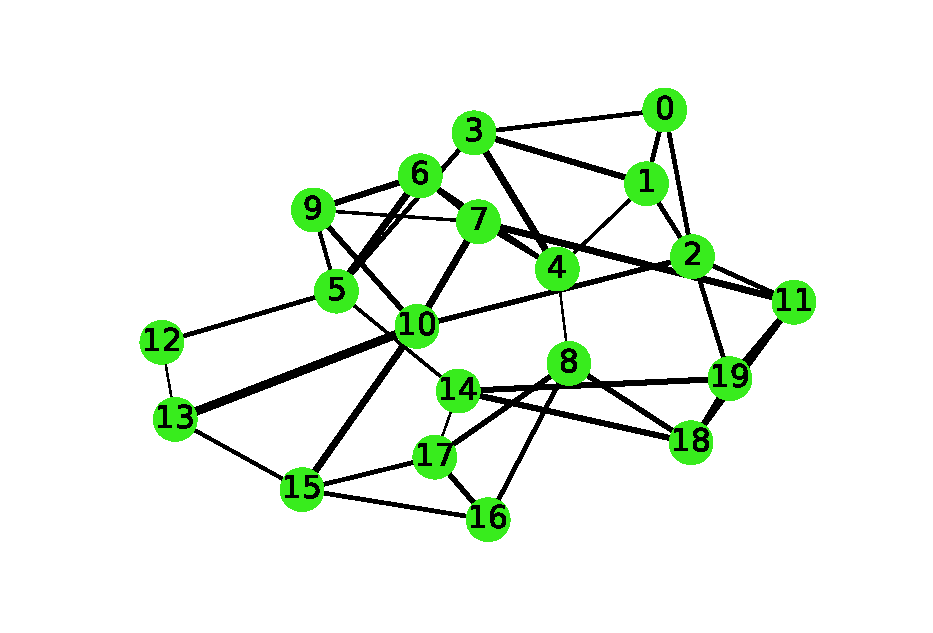
\includegraphics[scale=0.60]{fig1a.eps}}
\subfigure[\textit{Grafo 2}]{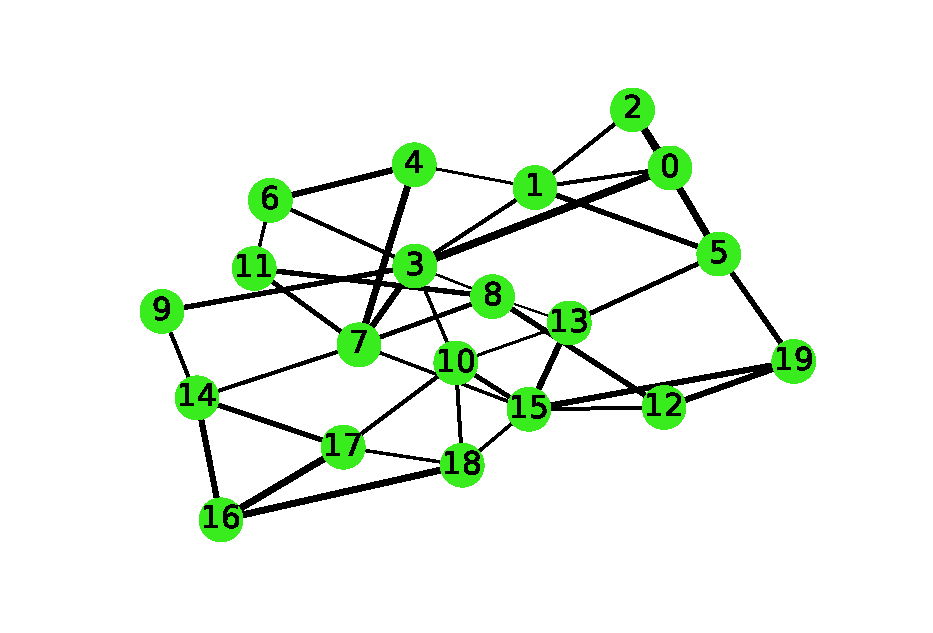
\includegraphics[scale=0.60]{fig2a.eps}}
\subfigure[\textit{Grafo 3}]{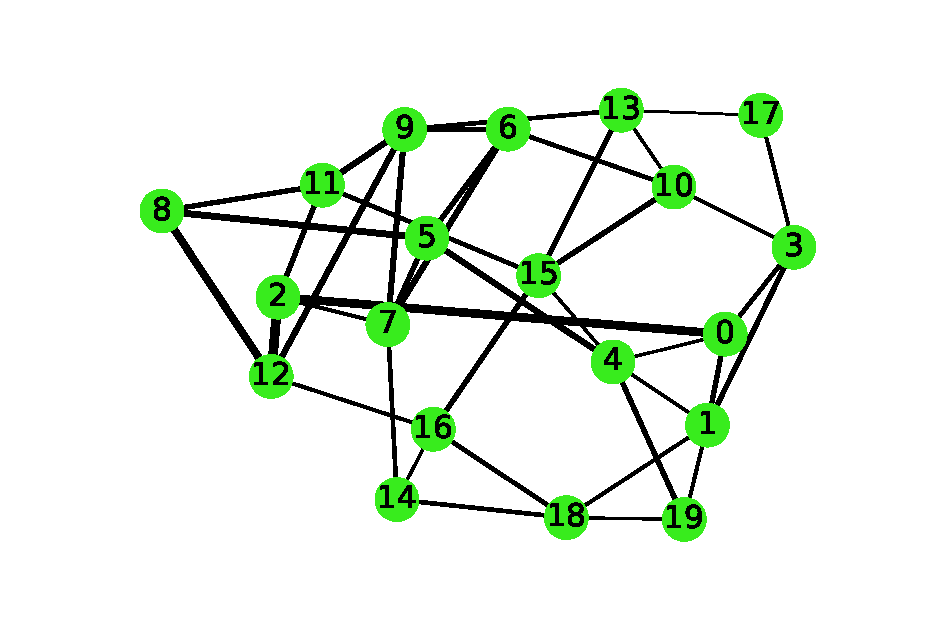
\includegraphics[scale=0.60]{fig3a.eps}}
\subfigure[\textit{Grafo 4}]{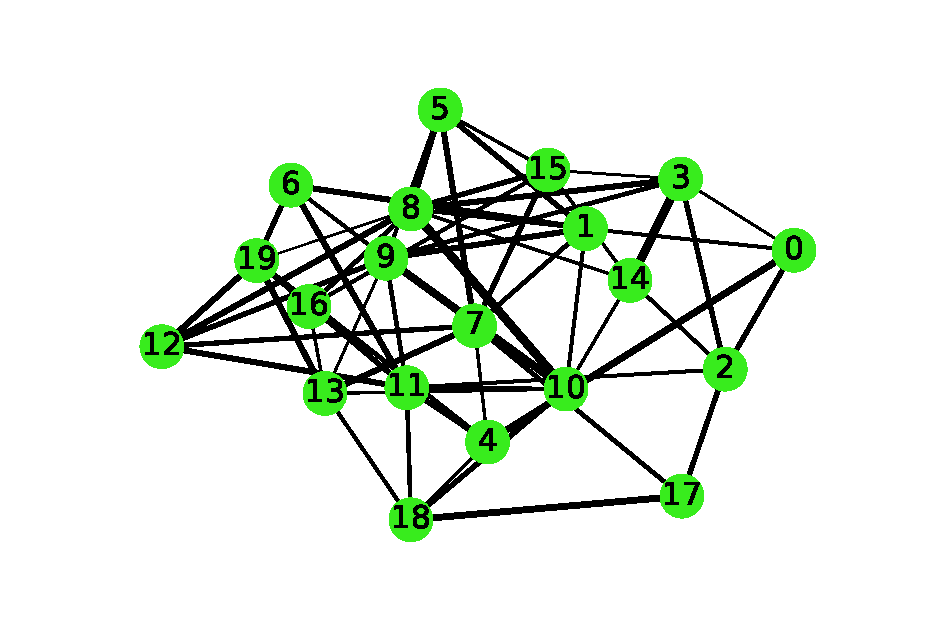
\includegraphics[scale=0.60]{fig4a.eps}}
\subfigure[\textit{Grafo 5}]{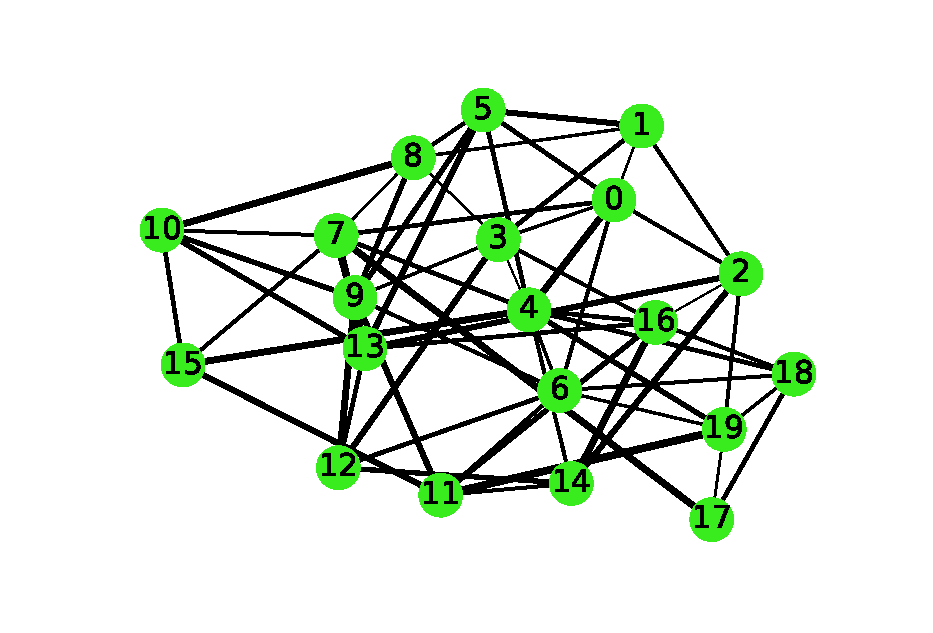
\includegraphics[scale=0.60]{fig5a.eps}}
\caption{Grafos generados}
\label{Fig1} 
\end{figure}

Luego se calcularon las propiedades para cada vértice de cada grafo usando el siguiente código:

\newpage
\lstinputlisting[language=Python, firstline=19, lastline=63]{T5histoporopiedad.py}

Para tener un avance del comportamiento de estas propiedades de los vértices las cuales se emplearan en el análsis de varianza más adelante, para cada grafo se realizaron los histogramas de cada una de las propiedades (distribución de grado, coeficiente de agrupamiento, centralidad de cercanía, centralidad de carga, excentricidad y \textit{pagerank}) por cada grafo. Los mismos se muestran a continuación:

Análisis del comportamiento de la distribución de grado en cada grafo. Ver figura \ref{Fig2} de la página \pageref{Fig2} 

\begin{figure}[htbp]
\subfigure[\textit{Grafo 1}]{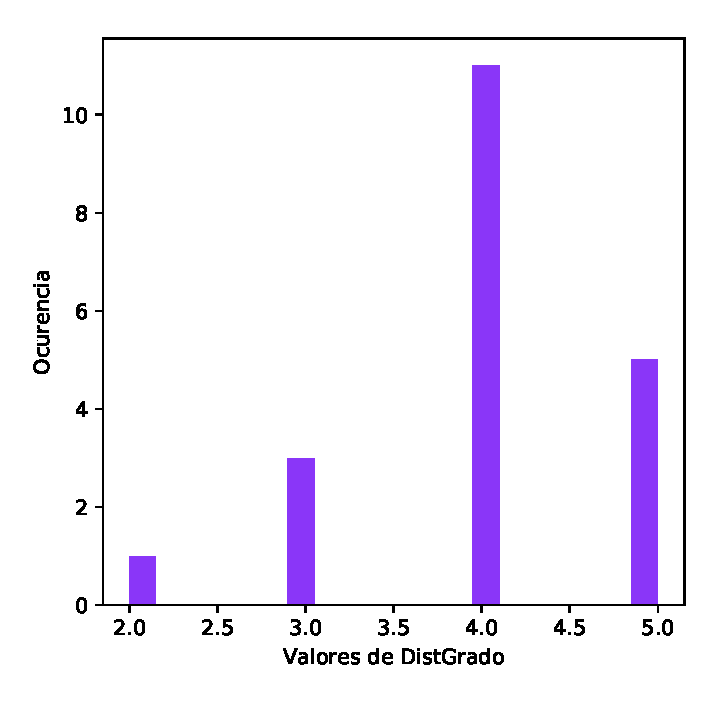
\includegraphics[scale=0.60]{histogramapropiedadesgrafo1DistGrado.eps}}
\subfigure[\textit{Grafo 2}]{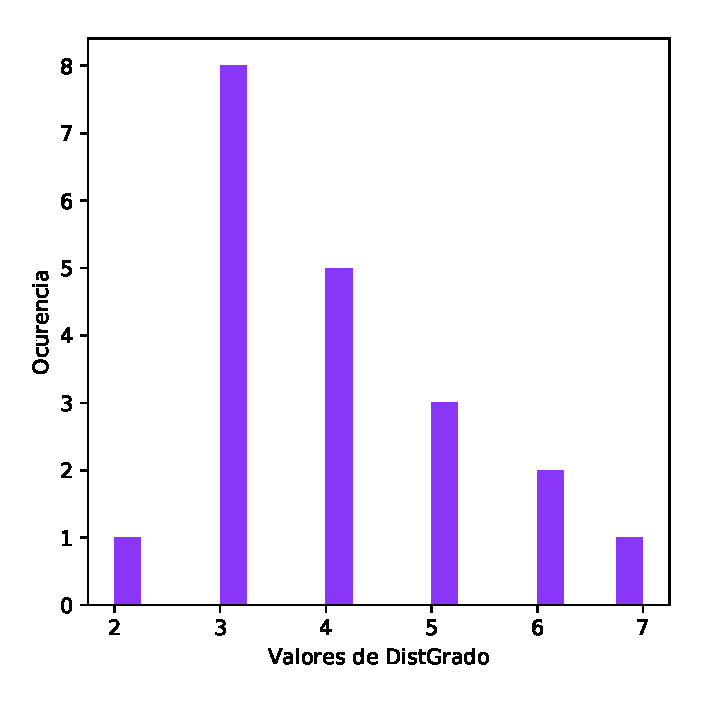
\includegraphics[scale=0.60]{histogramapropiedadesgrafo2DistGrado.eps}}
\subfigure[\textit{Grafo 3}]{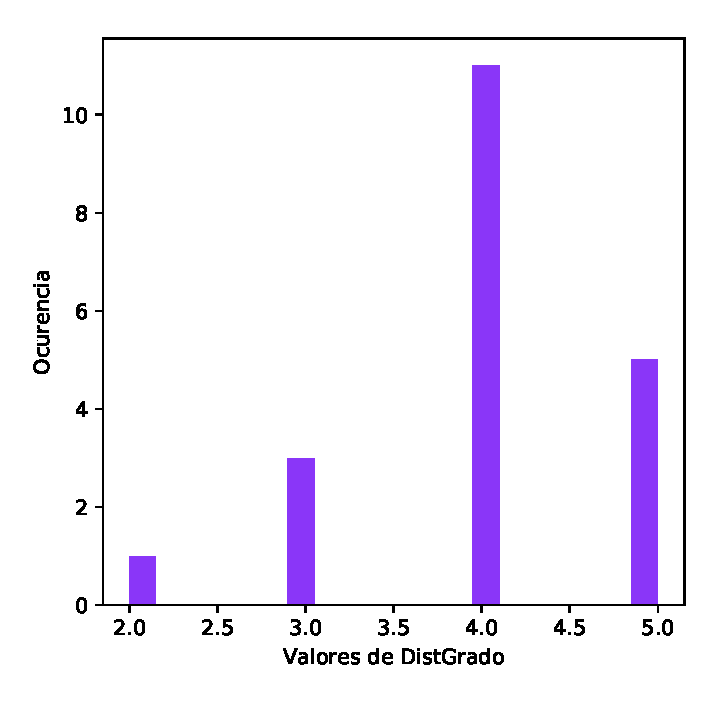
\includegraphics[scale=0.60]{histogramapropiedadesgrafo3DistGrado.eps}}
\subfigure[\textit{Grafo 4}]{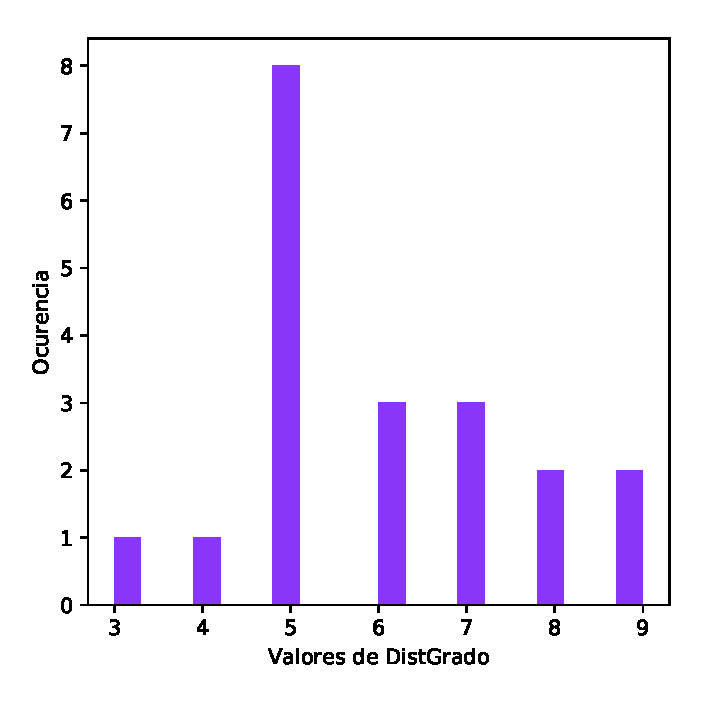
\includegraphics[scale=0.60]{histogramapropiedadesgrafo4DistGrado.eps}}
\subfigure[\textit{Grafo 5}]{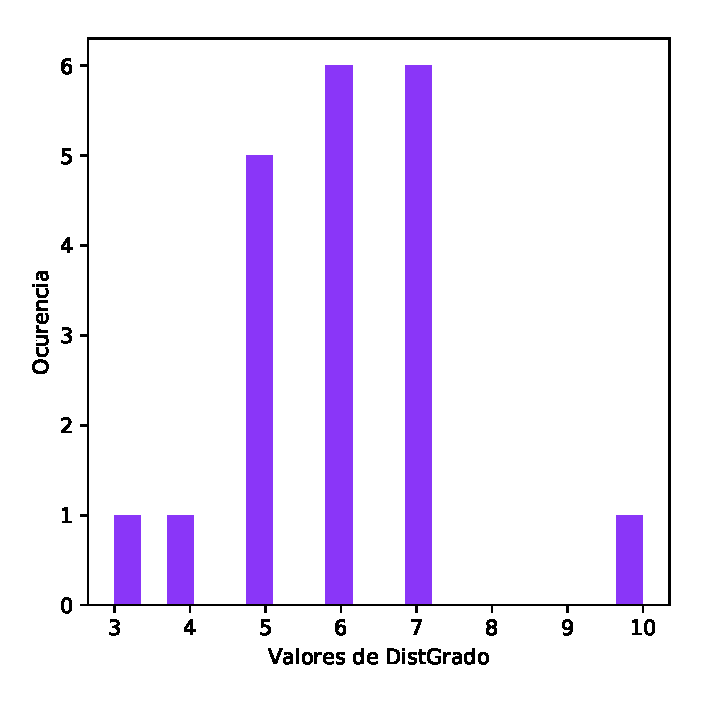
\includegraphics[scale=0.60]{histogramapropiedadesgrafo5DistGrado.eps}}
\caption{Histogramas de distribución de grado por grafo}
\label{Fig2} 
\end{figure}
\newpage
Análisis del comportamiento del coeficiente de agrupamiento. Ver figura \ref{Fig3} de la página \pageref{Fig3} 

\begin{figure}[htbp]
\subfigure[\textit{Grafo 1}]{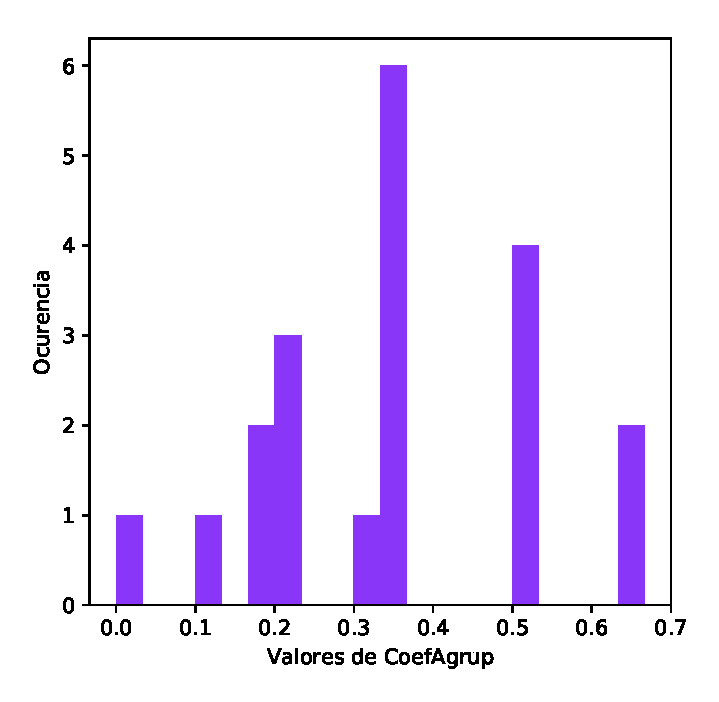
\includegraphics[scale=0.50, trim=0 0 0 10, clip=true]{histogramapropiedadesgrafo1CoefAgrup.eps}}
\subfigure[\textit{Grafo 2}]{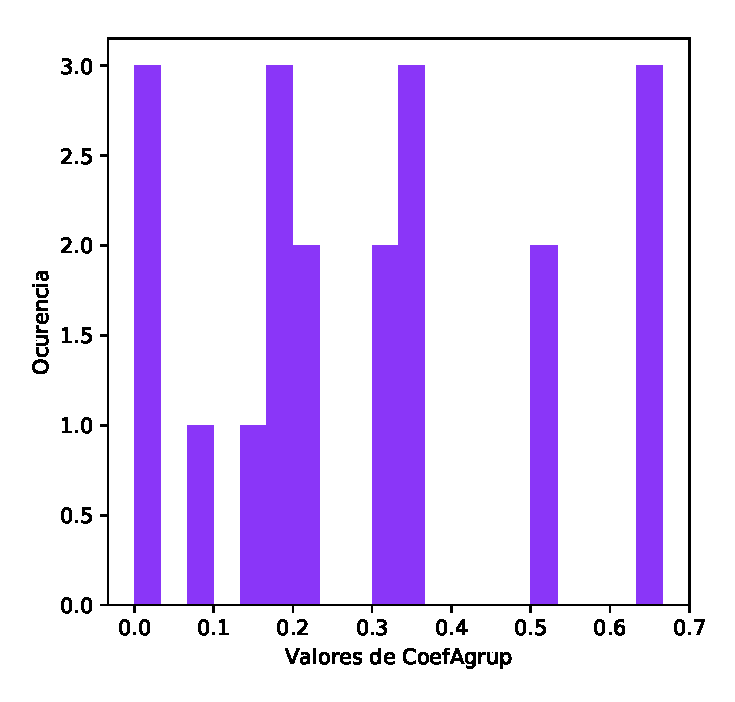
\includegraphics[scale=0.50, trim=0 0 0 10, clip=true]{histogramapropiedadesgrafo2CoefAgrup.eps}}
\subfigure[\textit{Grafo 3}]{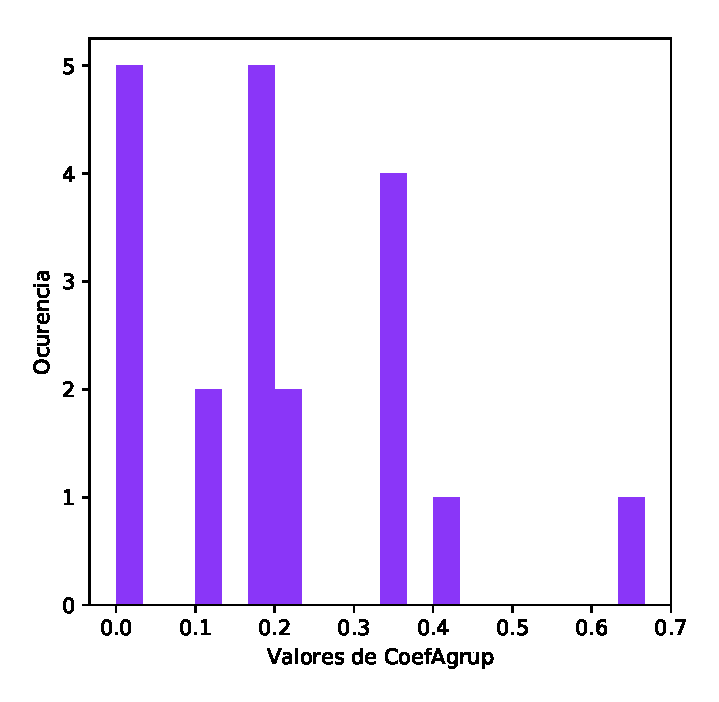
\includegraphics[scale=0.50, trim=0 0 0 10, clip=true]{histogramapropiedadesgrafo3CoefAgrup.eps}}
\subfigure[\textit{Grafo 4}]{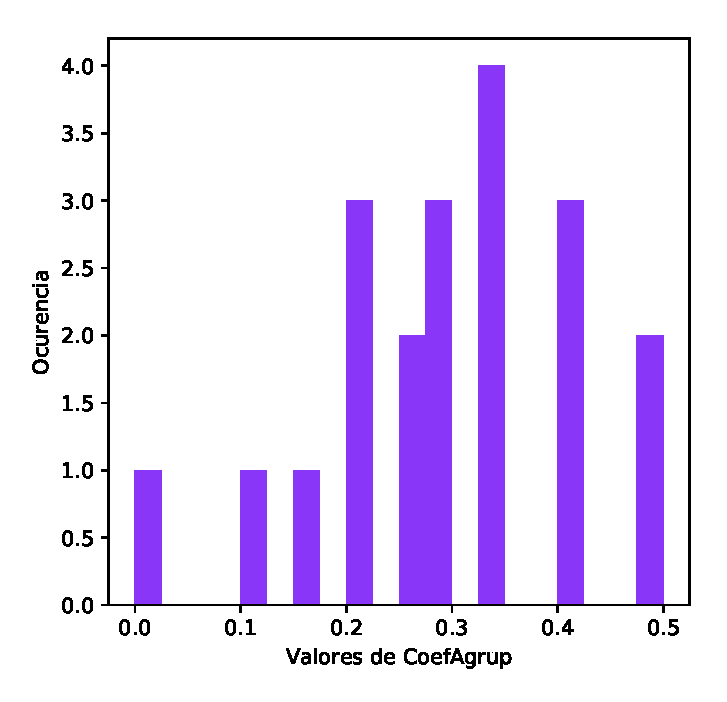
\includegraphics[scale=0.50, trim=0 0 0 10, clip=true]{histogramapropiedadesgrafo4CoefAgrup.eps}}
\subfigure[\textit{Grafo 5}]{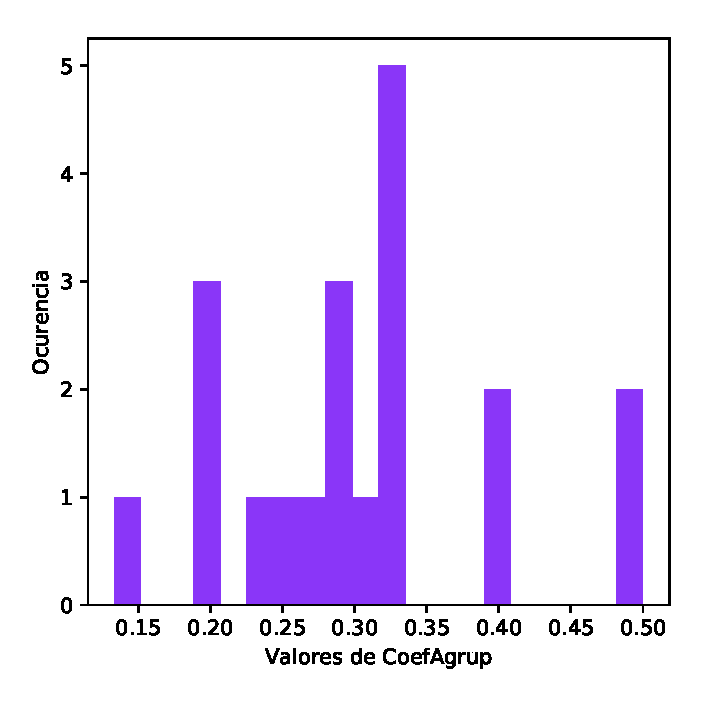
\includegraphics[scale=0.50, trim=0 0 0 10, clip=true]{histogramapropiedadesgrafo5CoefAgrup.eps}}
\caption{Histogramas del coeficiente de agrupamiento por grafo}
\label{Fig3} 
\end{figure}


Análisis del comportamiento de la centralidad de cercanía en cada grafo. Ver figura \ref{Fig4} de la página \pageref{Fig4} 

\begin{figure}[htbp]
\subfigure[\textit{Grafo 1}]{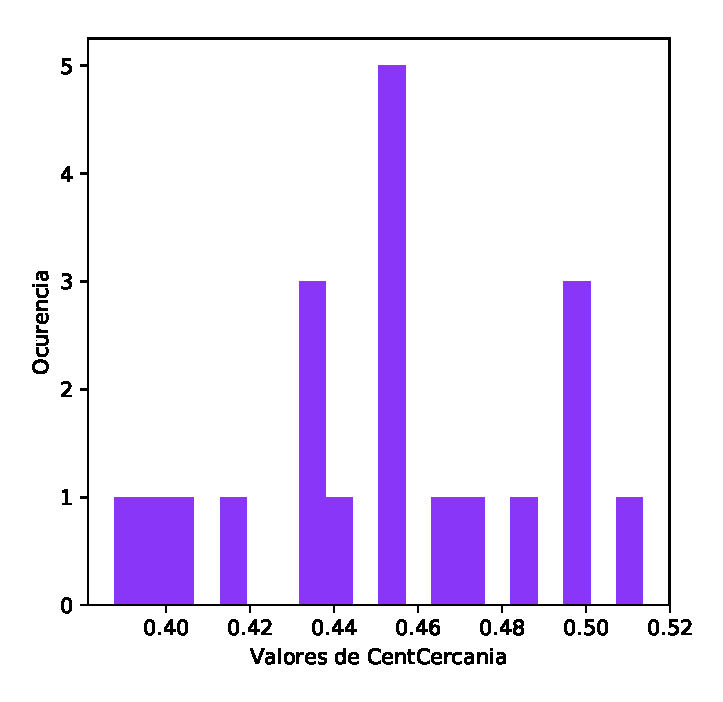
\includegraphics[scale=0.60, trim=0 0 0 10, clip=true]{histogramapropiedadesgrafo1CentCercania.eps}}
\subfigure[\textit{Grafo 2}]{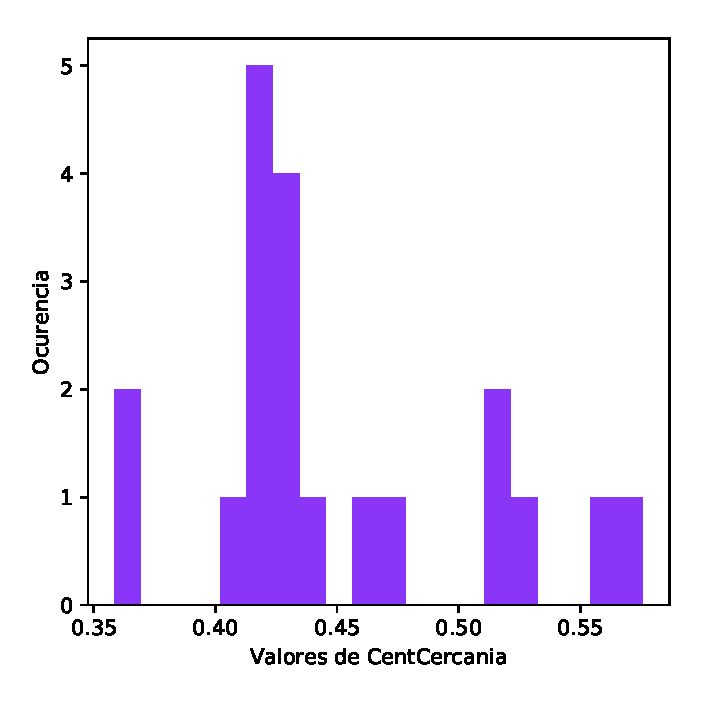
\includegraphics[scale=0.60, trim=0 0 0 10, clip=true]{histogramapropiedadesgrafo2CentCercania.eps}}
\subfigure[\textit{Grafo 3}]{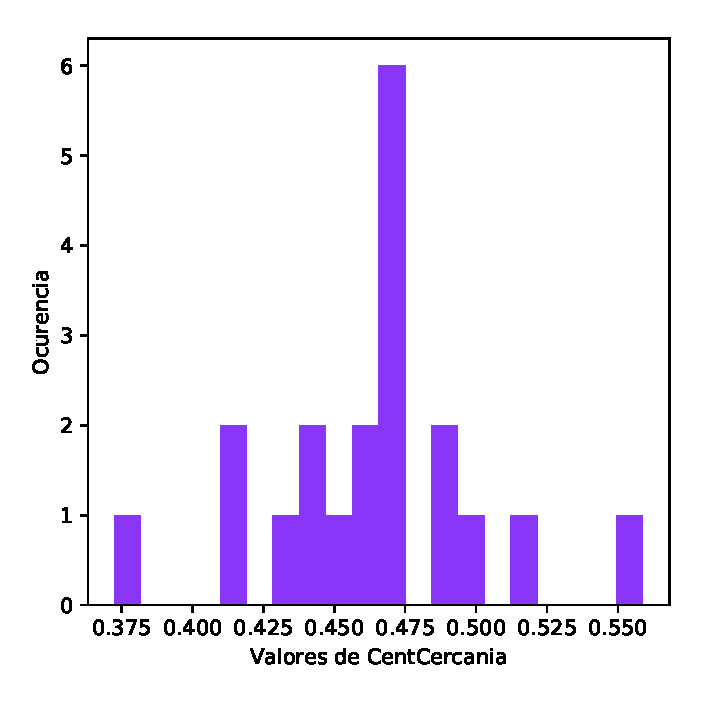
\includegraphics[scale=0.60, trim=0 0 0 10, clip=true]{histogramapropiedadesgrafo3CentCercania.eps}}
\subfigure[\textit{Grafo 4}]{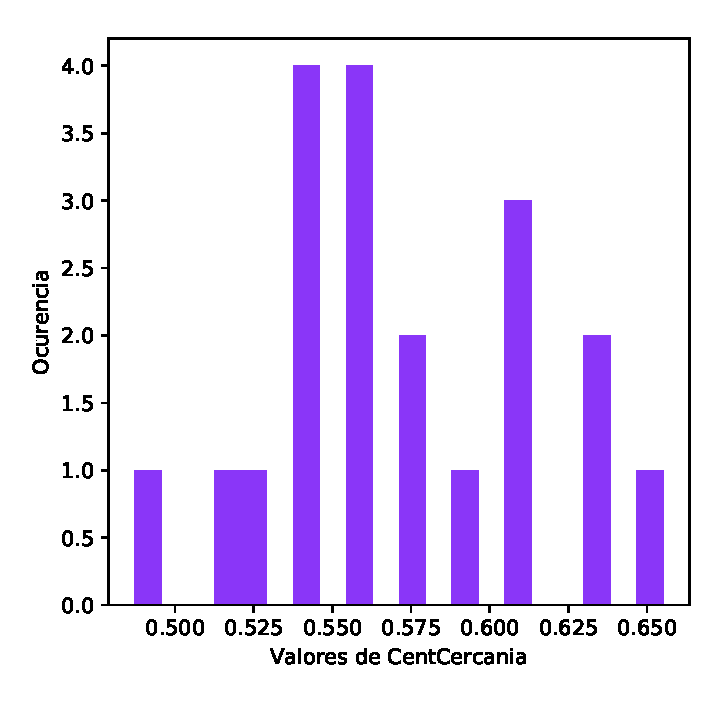
\includegraphics[scale=0.60, trim=0 0 0 10, clip=true]{histogramapropiedadesgrafo4CentCercania.eps}}
\subfigure[\textit{Grafo 5}]{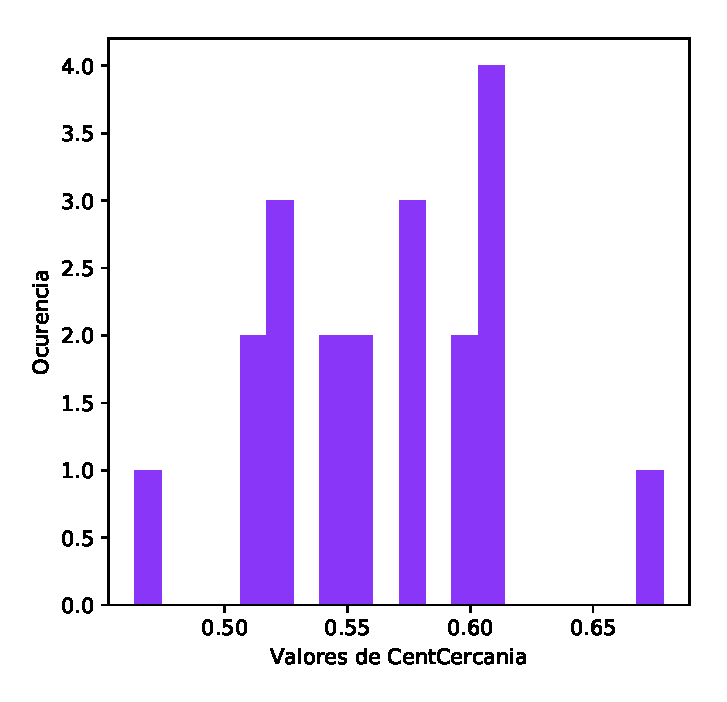
\includegraphics[scale=0.60, trim=0 0 0 10, clip=true]{histogramapropiedadesgrafo5CentCercania.eps}}
\caption{Histogramas de la centralidad de cercanía}
\label{Fig4} 
\end{figure}

Análisis del comportamiento de la centralidad de carga en cada grafo. Ver figura \ref{Fig5} de la página \pageref{Fig5} 

\begin{figure}[htbp]
\subfigure[\textit{Grafo 1}]{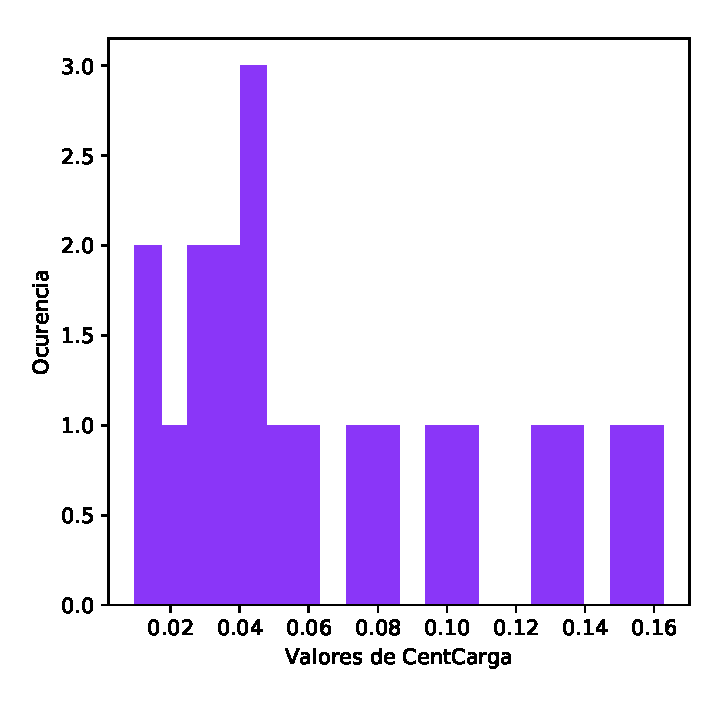
\includegraphics[scale=0.60]{histogramapropiedadesgrafo1CentCarga.eps}}
\subfigure[\textit{Grafo 2}]{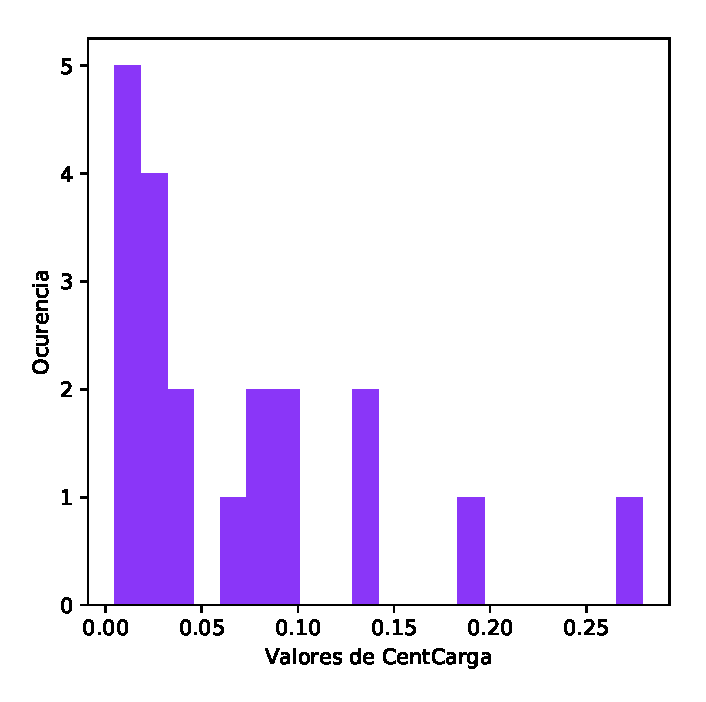
\includegraphics[scale=0.60]{histogramapropiedadesgrafo2CentCarga.eps}}
\subfigure[\textit{Grafo 3}]{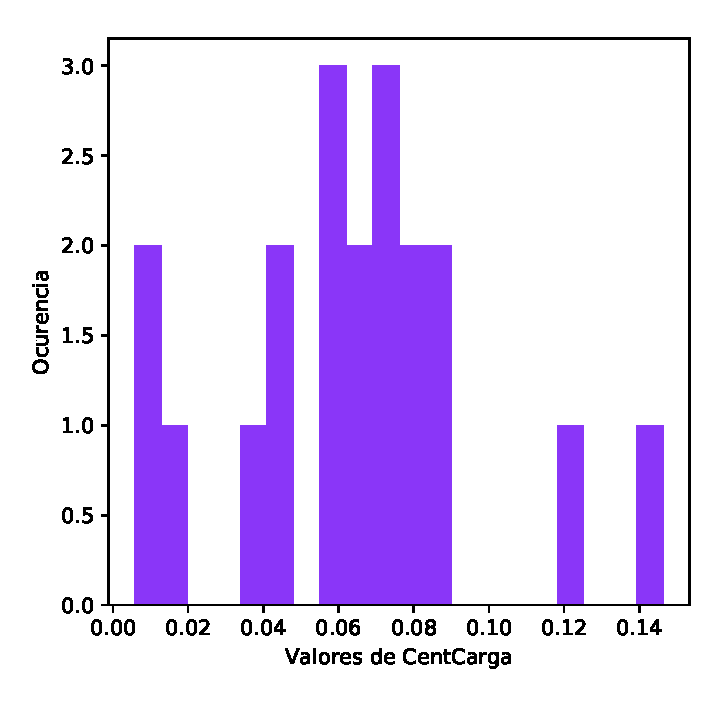
\includegraphics[scale=0.60]{histogramapropiedadesgrafo3CentCarga.eps}}
\subfigure[\textit{Grafo 4}]{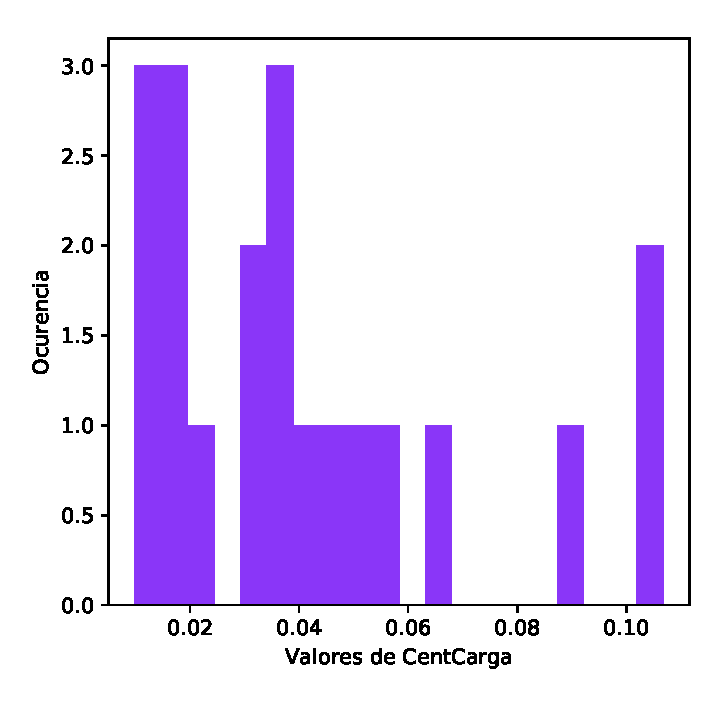
\includegraphics[scale=0.60]{histogramapropiedadesgrafo4CentCarga.eps}}
\subfigure[\textit{Grafo 5}]{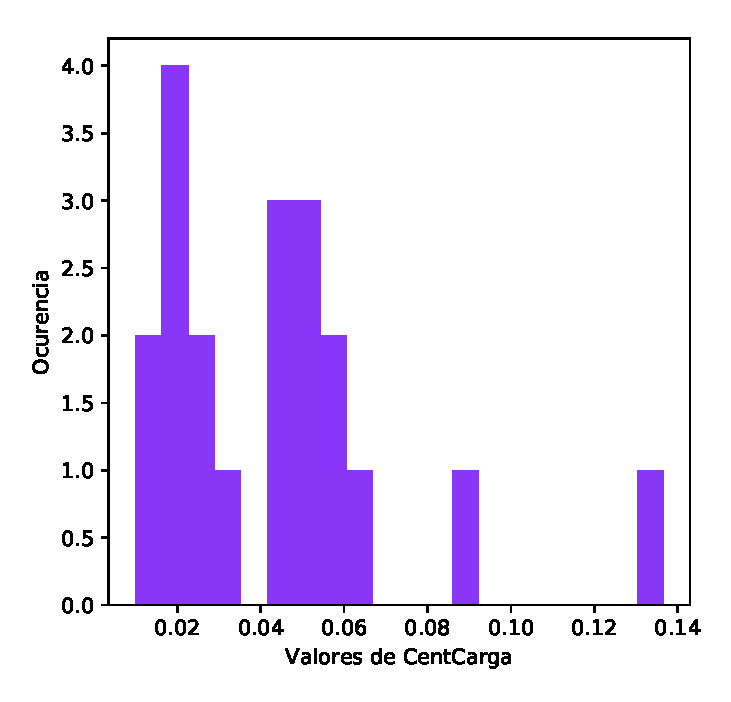
\includegraphics[scale=0.60]{histogramapropiedadesgrafo5CentCarga.eps}}
\caption{Histogramas de la centralidad de carga}
\label{Fig5} 
\end{figure}

Análisis del comportamiento de la excentricidad en cada grafo. Ver figura \ref{Fig6} de la página \pageref{Fig6} 

\begin{figure}[htbp]
\subfigure[\textit{Grafo 1}]{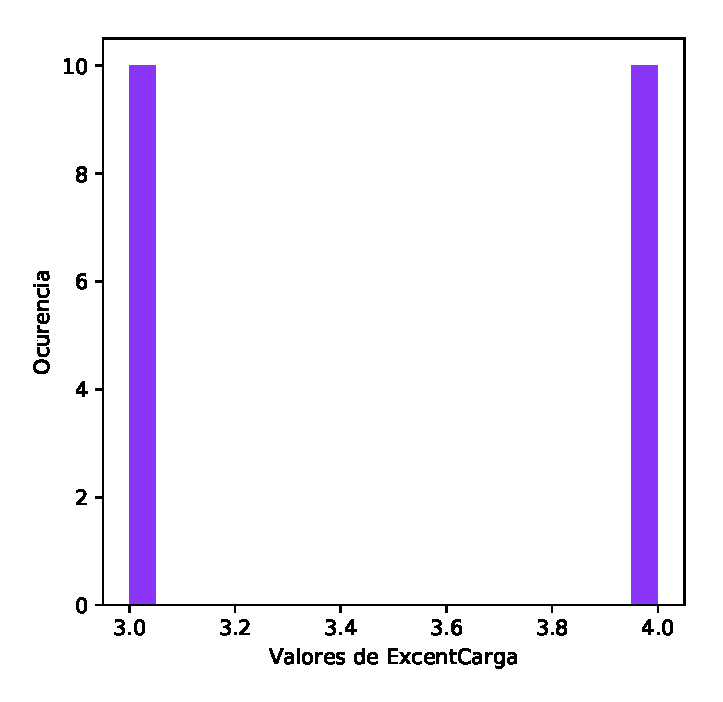
\includegraphics[scale=0.60]{histogramapropiedadesgrafo1ExcentCarga.eps}}
\subfigure[\textit{Grafo 2}]{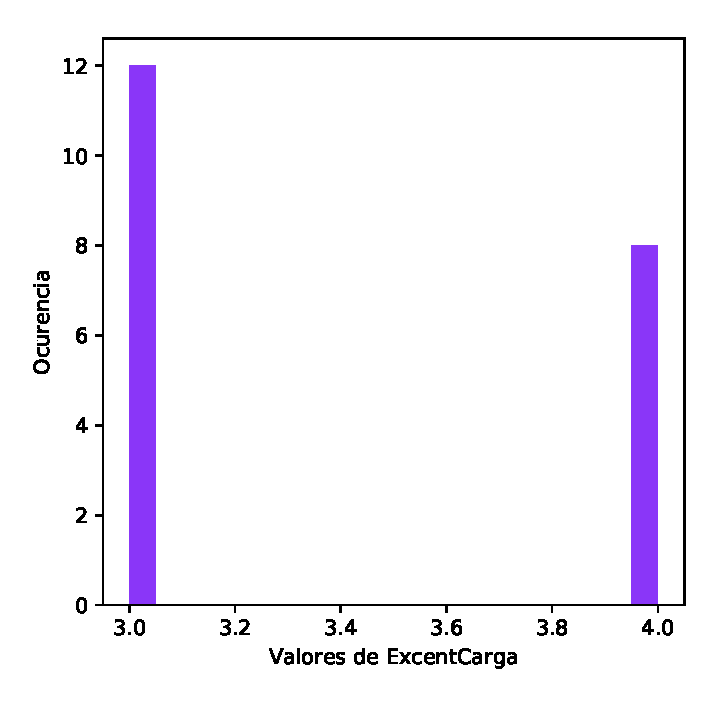
\includegraphics[scale=0.60]{histogramapropiedadesgrafo3ExcentCarga.eps}}
\subfigure[\textit{Grafo 3}]{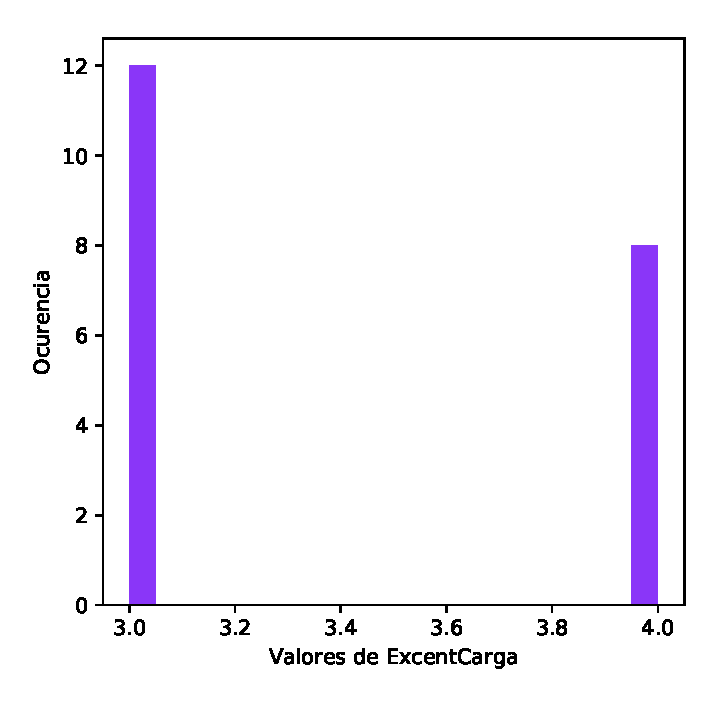
\includegraphics[scale=0.60]{histogramapropiedadesgrafo3ExcentCarga.eps}}
\subfigure[\textit{Grafo 4}]{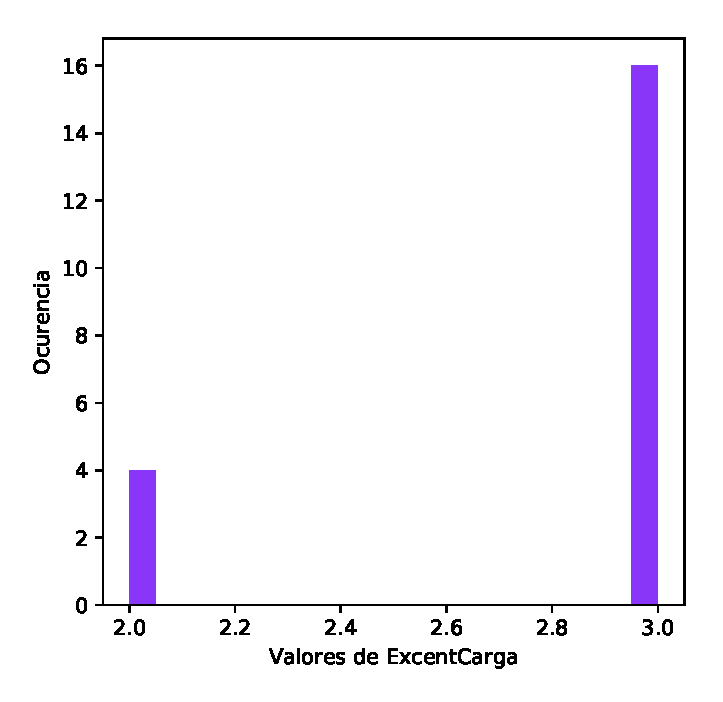
\includegraphics[scale=0.60]{histogramapropiedadesgrafo4ExcentCarga.eps}}
\subfigure[\textit{Grafo 5}]{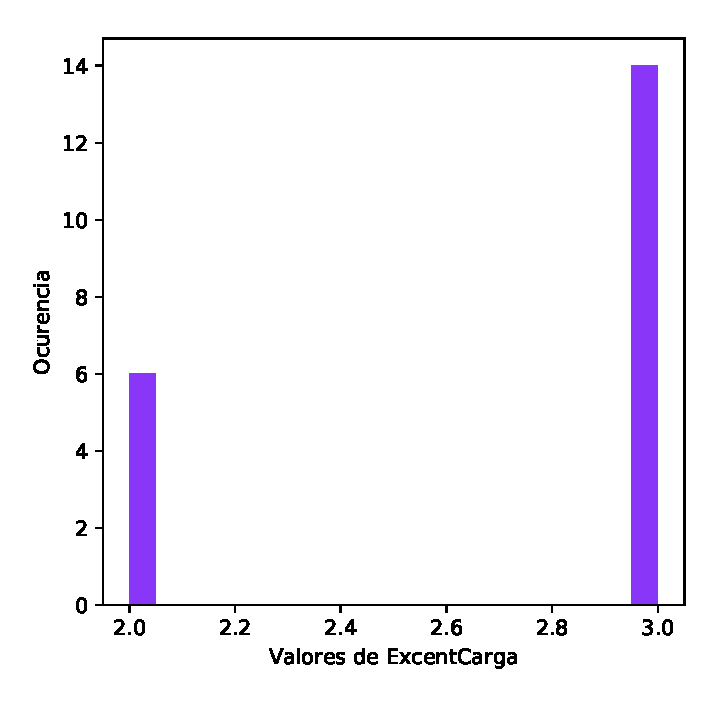
\includegraphics[scale=0.60]{histogramapropiedadesgrafo5ExcentCarga.eps}}
\caption{Histogramas de la excentricidad}
\label{Fig6} 
\end{figure}

Análisis del comportamiento del \textit{pagerank} en cada grafo. Ver figura \ref{Fig7} de la página \pageref{Fig7} 

\begin{figure}[htbp]
\subfigure[\textit{Grafo 1}]{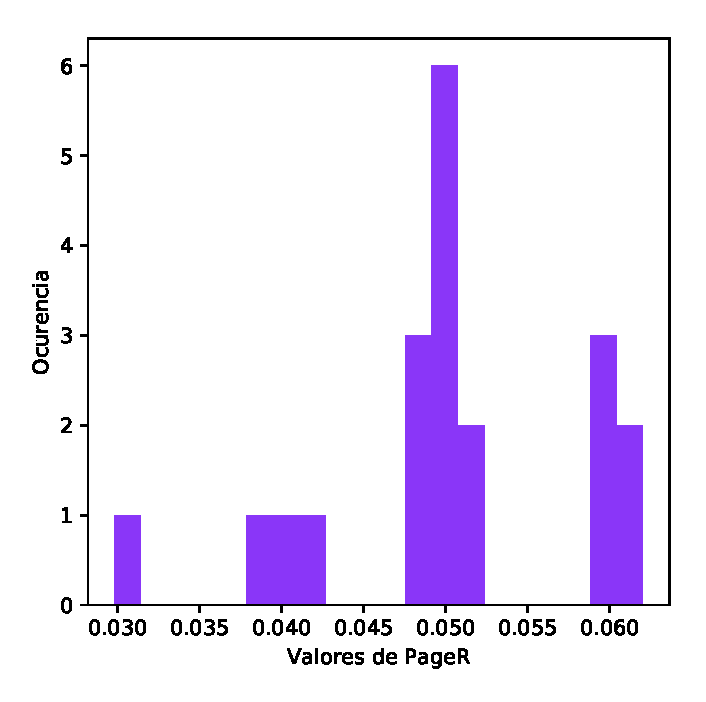
\includegraphics[scale=0.60]{histogramapropiedadesgrafo1PageR.eps}}
\subfigure[\textit{Grafo 2}]{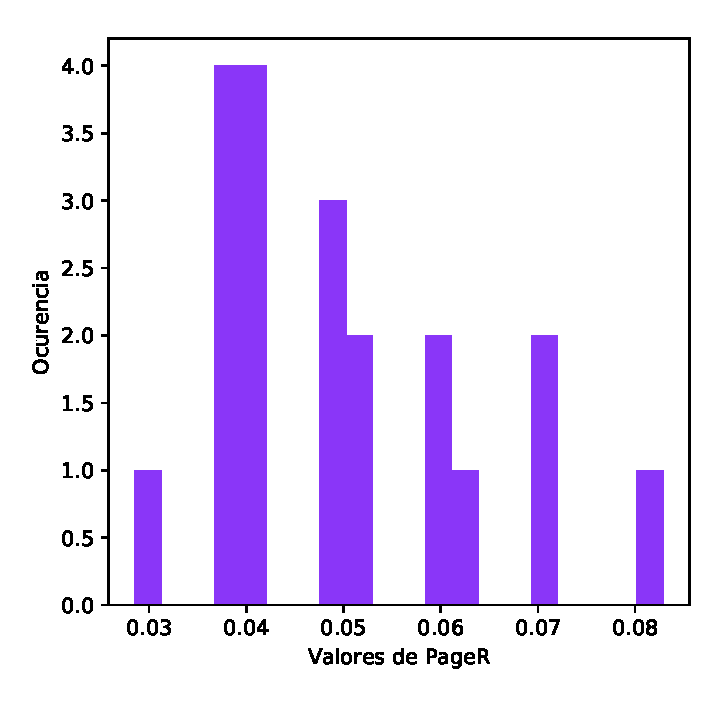
\includegraphics[scale=0.60]{histogramapropiedadesgrafo2PageR.eps}}
\subfigure[\textit{Grafo 3}]{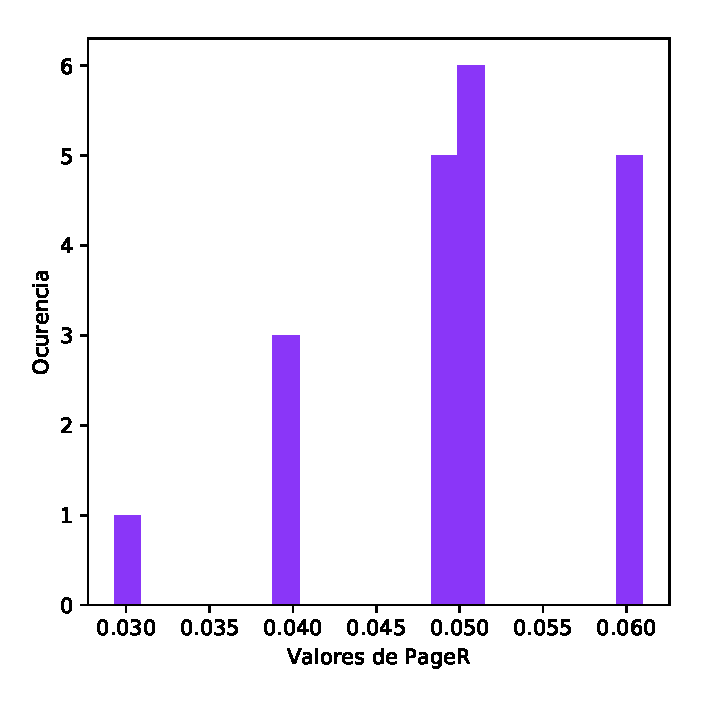
\includegraphics[scale=0.60]{histogramapropiedadesgrafo3PageR.eps}}
\subfigure[\textit{Grafo 4}]{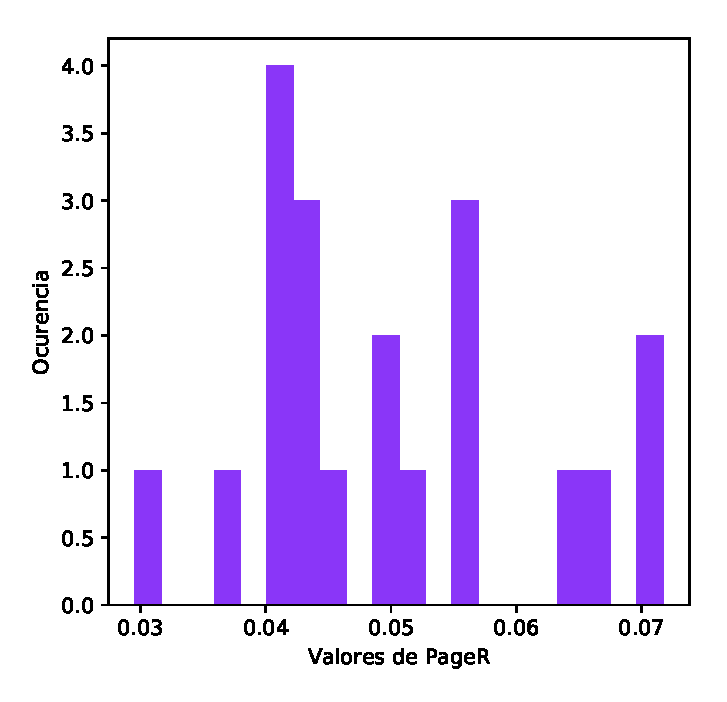
\includegraphics[scale=0.60]{histogramapropiedadesgrafo4PageR.eps}}
\subfigure[\textit{Grafo 5}]{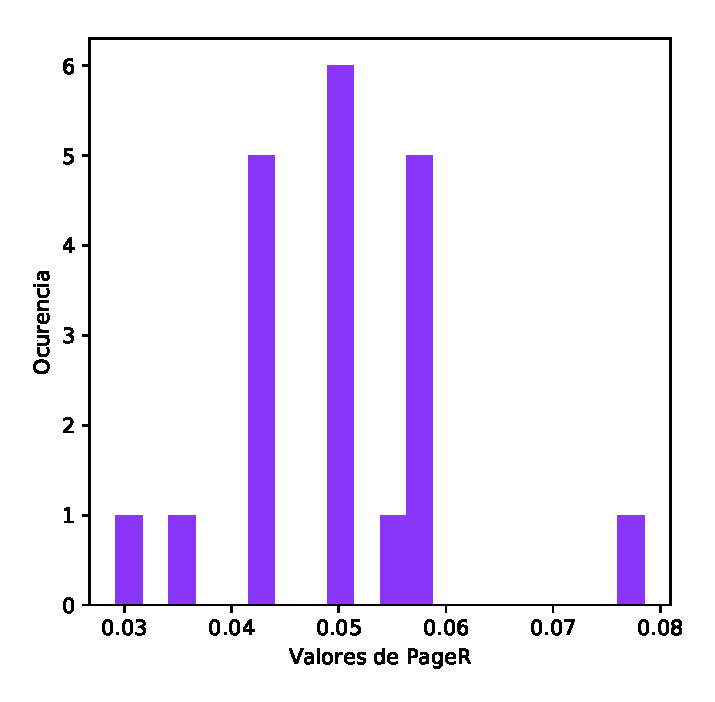
\includegraphics[scale=0.60]{histogramapropiedadesgrafo5PageR.eps}}
\caption{Histogramas del \textit{pagerank}}
\label{Fig7} 
\end{figure}
\newpage
Al observar el comportamiento de estas variables se aprecia que no describen una distribución normal, por lo que no es recomendable hacer el análisis de varianza de influencia en el tiempo de ejecución del algoritmo y el flujo máximo usando el promedio, sino la mediana.

Para realizar el cálculo del tiempo de ejecución del algoritmo y el flujo máximo variando los nodos fuentes y sumideros de modo que toda la información quedase guardada en un .csv que pudiera emplearse en el análisis de varianza (ANOVA) se usó el siguiente código:


\lstinputlisting[language=Python, firstline=32, lastline=90]{T5Paraunircsvfinal.py}

\section{Influencia en el óptimo al variar nodos fuentes y sumideros} 

Al variar los nodos fuentes y sumideros fue calculado el valor de flujo máximo que se obtenía en cada caso, evidenciándose que existe variación en el óptimo para cada uno de los cinco grafos. A continuación se muestra para cada uno de los cinco grafos generados inicialmente el grafo inicial con la propuesta de mejor y peor fuente y sumidero. La fuente aparece con color rojo y el sumidero con color azul. De igual modo se emplea el degradado de color rojo para representar con rojo más intenso la mayor cantidad de flujo y más claro la menor cantidad de flujo que pasa por las aristas de la red residual que devuelve el algoritmo de flujo máximo seleccionado.

En la figura \ref{Fig12} de la página \pageref{Fig12} se observa la variación realizada para el grafo uno, en la figura \ref{Fig13} de la página \pageref{Fig13} la variación del grafo dos, en la figura \ref{Fig14} de la página \pageref{Fig14} la variación del grafo tres, en la figura \ref{Fig15} de la página \pageref{Fig15} la variación del grafo cuatro y figura \ref{Fig16} de la página \pageref{Fig16} la variación del grafo cinco.  

\begin{figure}[htbp]
\subfigure[\textit{Sin flujo}]{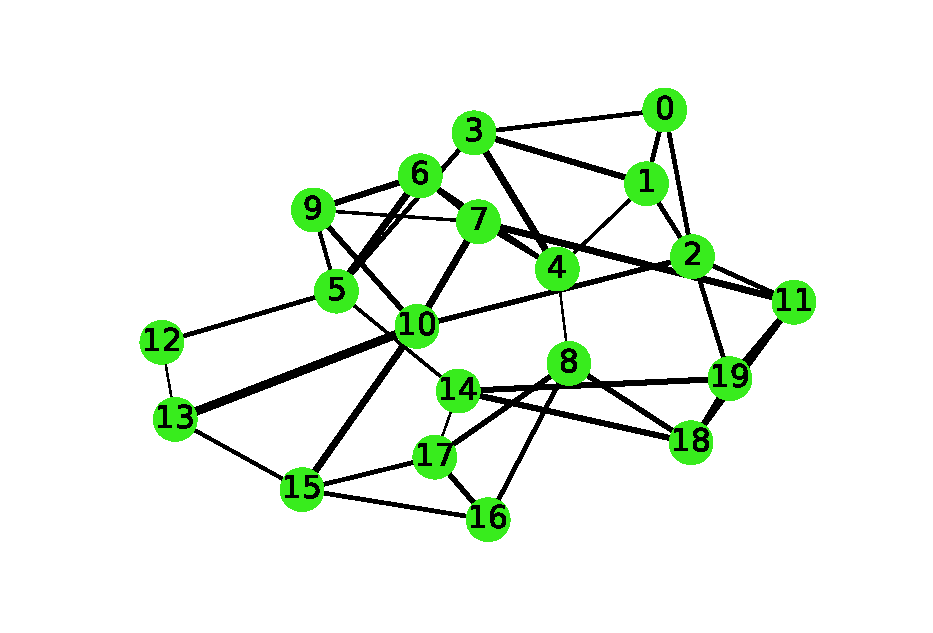
\includegraphics[scale=0.50]{fig1a.eps}}
\subfigure[\textit{Flujo máximo 59u }]{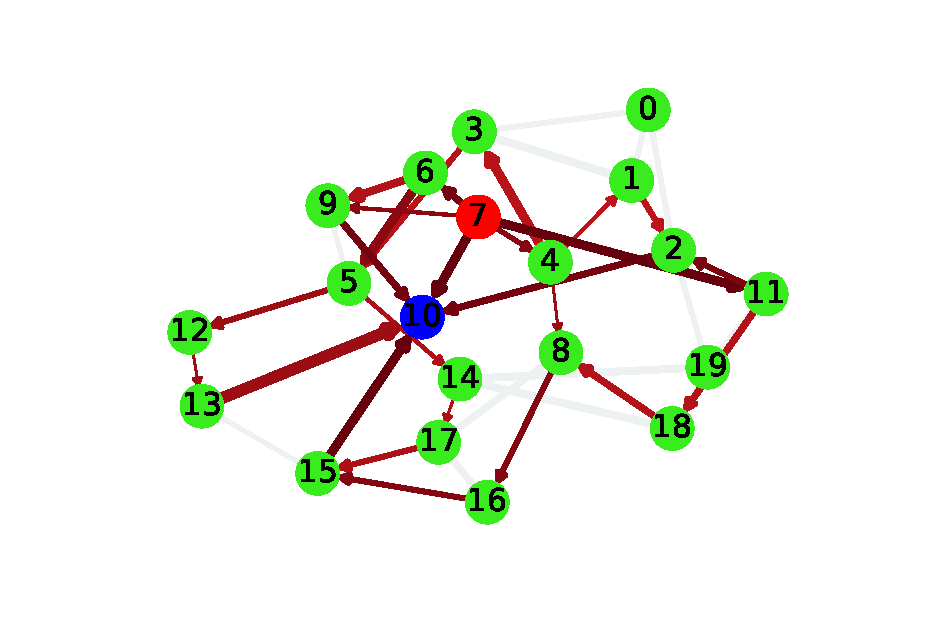
\includegraphics[scale=0.50]{fig1b1.eps}}
\subfigure[\textit{Flujo mínimo 18u }]{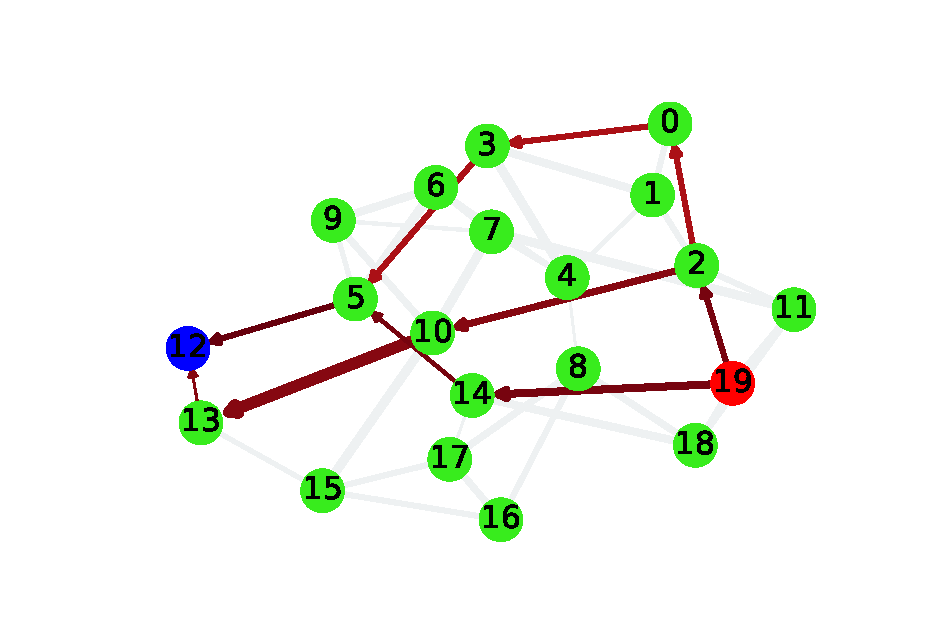
\includegraphics[scale=0.50]{fig1bpeor.eps}}
\caption{Variación de fuente y sumidero en grafo 1}
\label{Fig12} 
\end{figure}

\begin{figure}[htbp]
\subfigure[\textit{Sin flujo}]{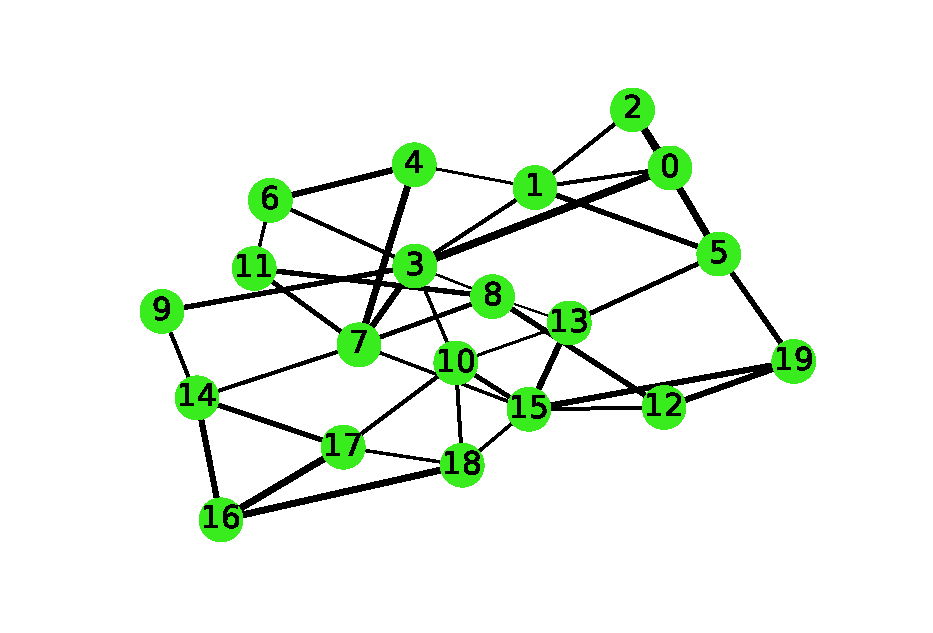
\includegraphics[scale=0.50]{fig2a.eps}}
\subfigure[\textit{Flujo máximo 68u }]{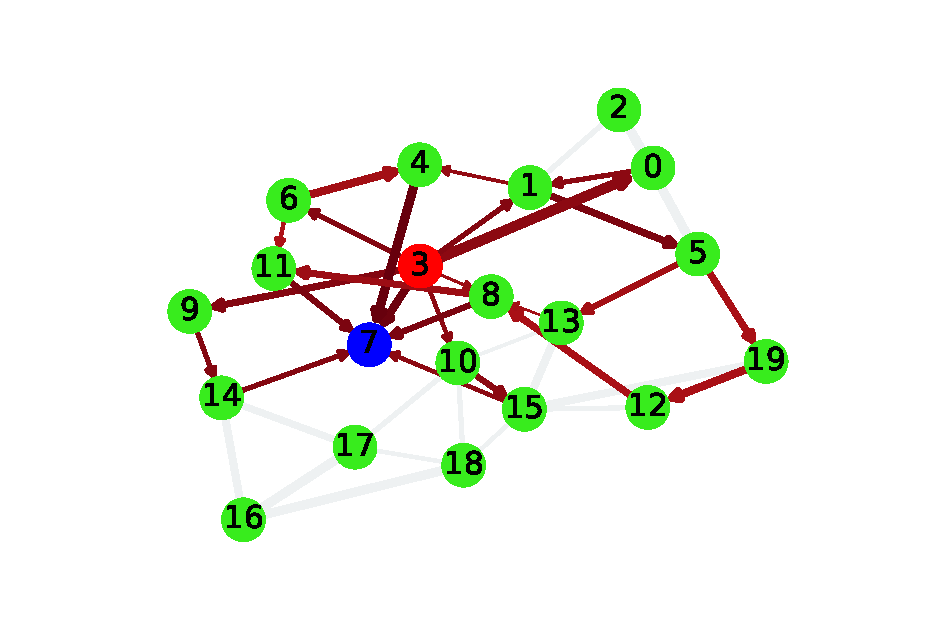
\includegraphics[scale=0.50]{fig2b1.eps}}
\subfigure[\textit{Flujo mínimo 22u }]{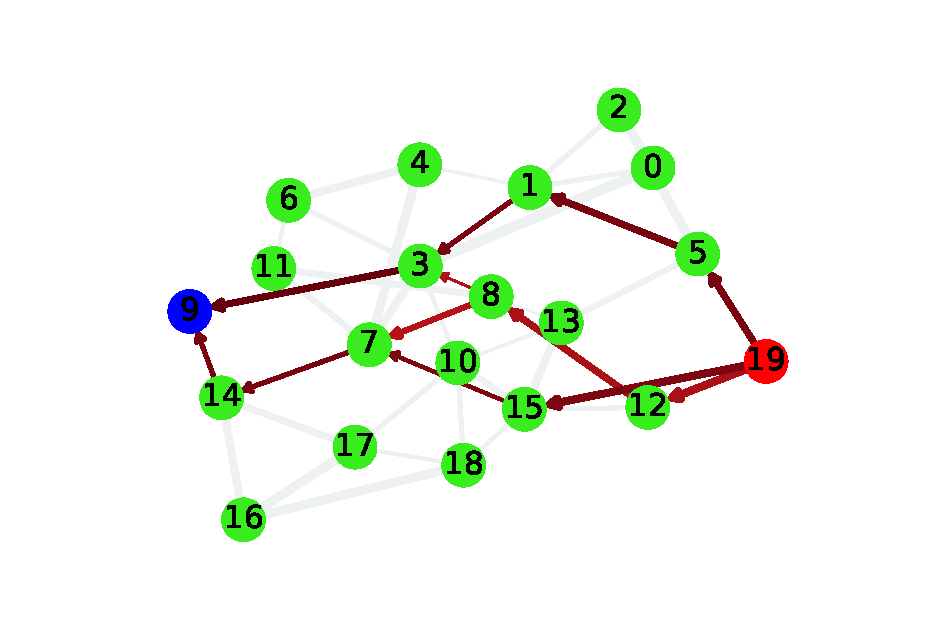
\includegraphics[scale=0.50]{fig2bpeor.eps}}
\caption{Variación de fuente y sumidero en grafo 2}
\label{Fig13} 
\end{figure}


\begin{figure}[htbp]
\subfigure[\textit{Sin flujo}]{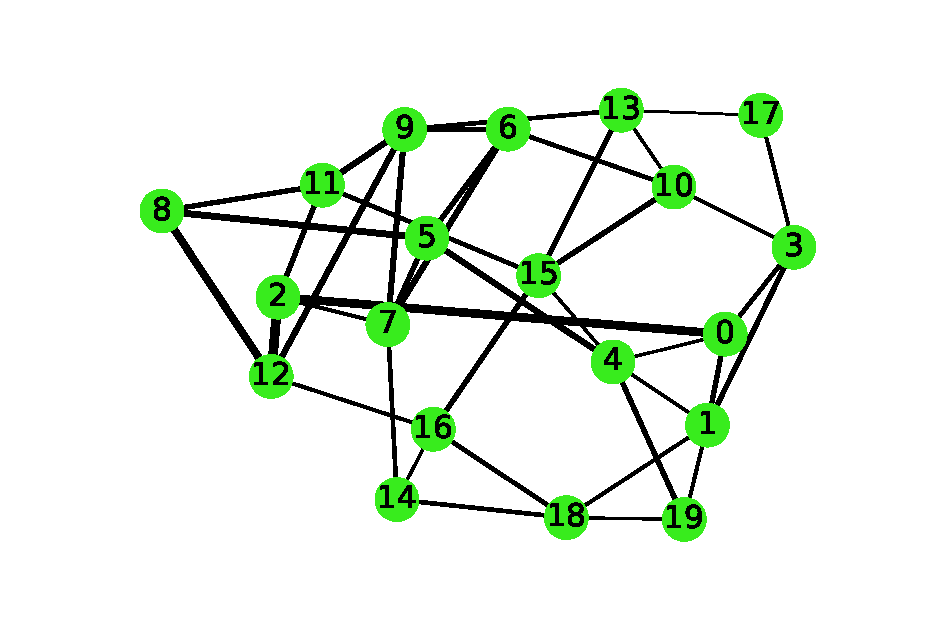
\includegraphics[scale=0.50]{fig3a.eps}}
\subfigure[\textit{Flujo máximo 59u }]{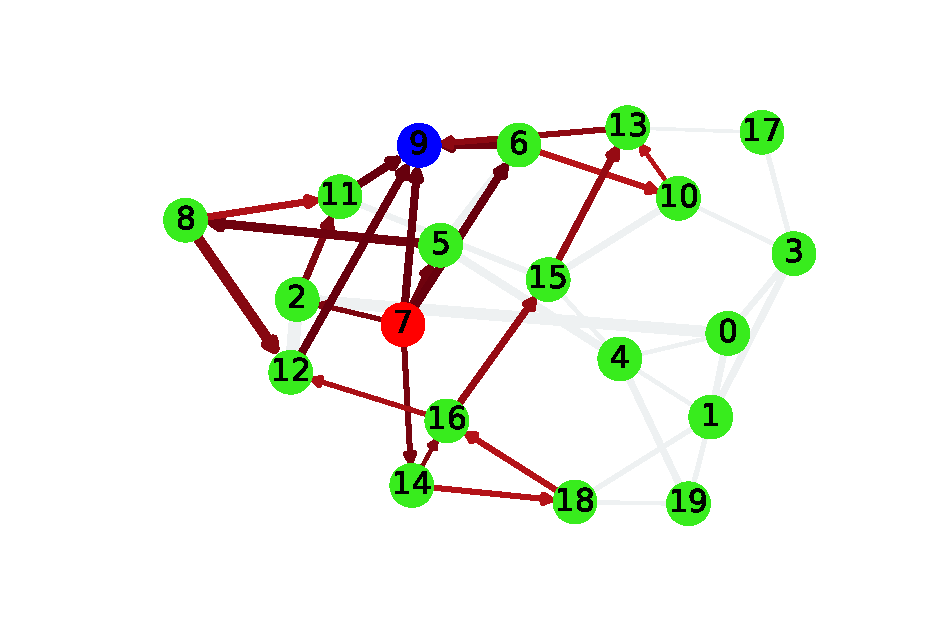
\includegraphics[scale=0.50]{fig3b1.eps}}
\subfigure[\textit{Flujo mínimo 18u }]{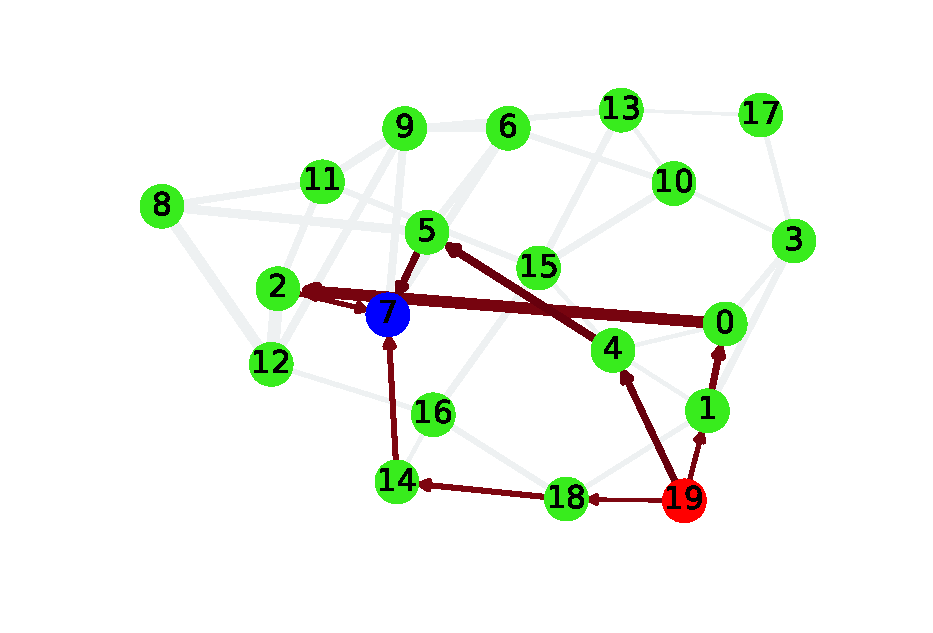
\includegraphics[scale=0.50]{fig3bpeor.eps}}
\caption{Variación de fuente y sumidero en grafo 3}
\label{Fig14} 
\end{figure}

\begin{figure}[htbp]
\subfigure[\textit{Sin flujo}]{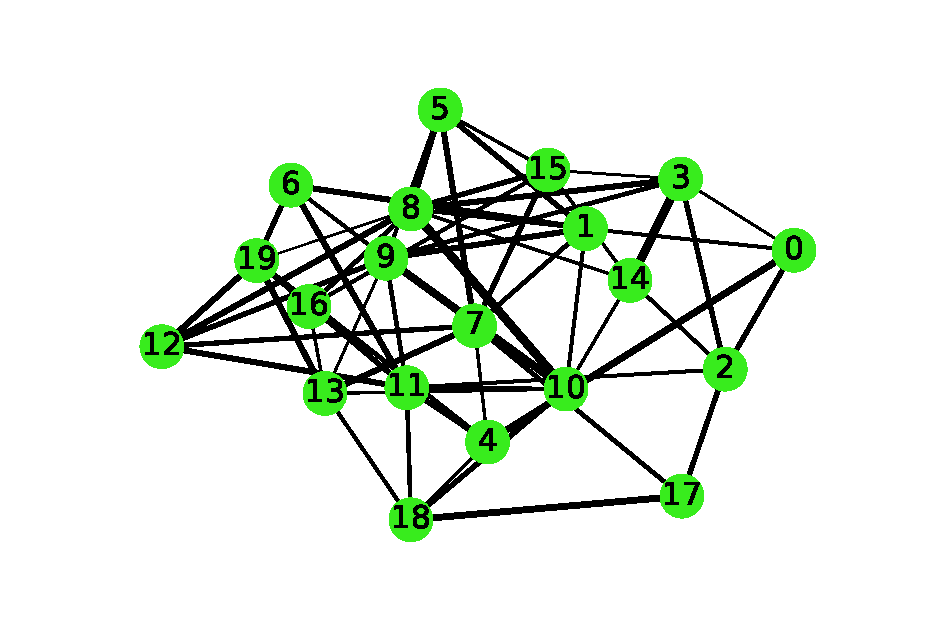
\includegraphics[scale=0.50]{fig4a.eps}}
\subfigure[\textit{Flujo máximo 102u }]{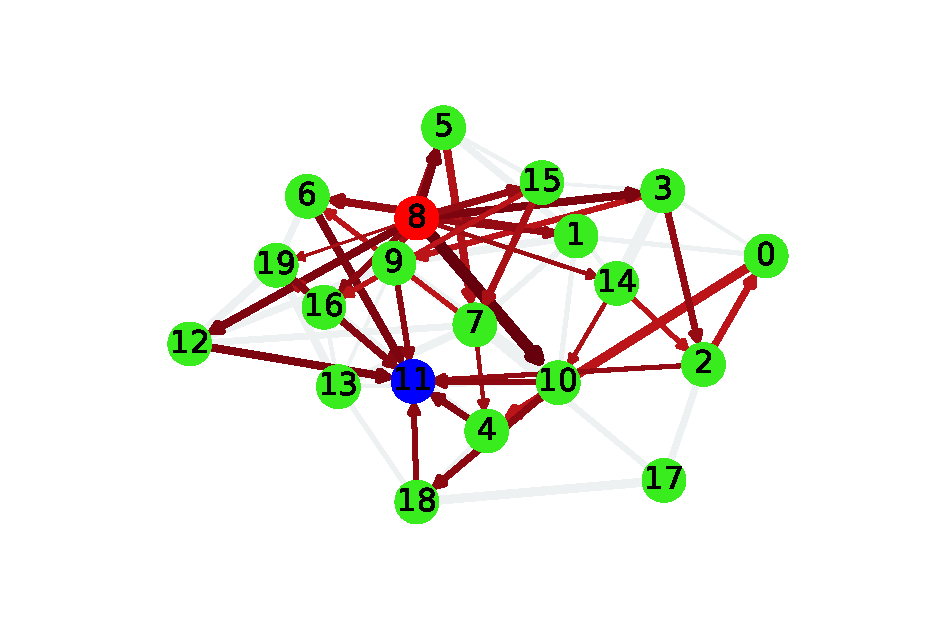
\includegraphics[scale=0.50]{fig4b1.eps}}
\subfigure[\textit{Flujo mínimo 37u }]{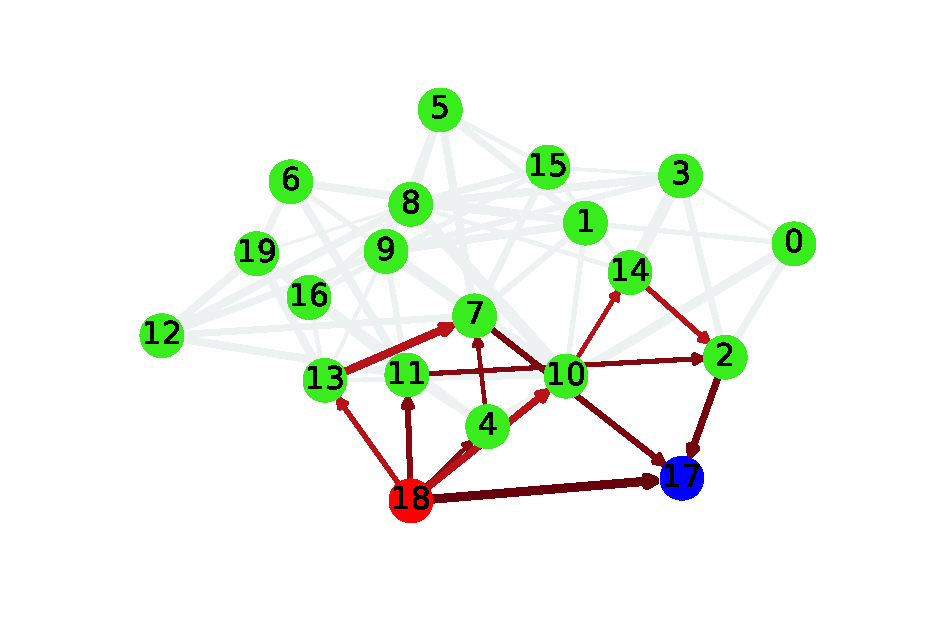
\includegraphics[scale=0.50]{fig4bpeor.eps}}
\caption{Variación de fuente y sumidero en grafo 4}
\label{Fig15} 
\end{figure}

\begin{figure}[htbp]
\subfigure[\textit{Sin flujo}]{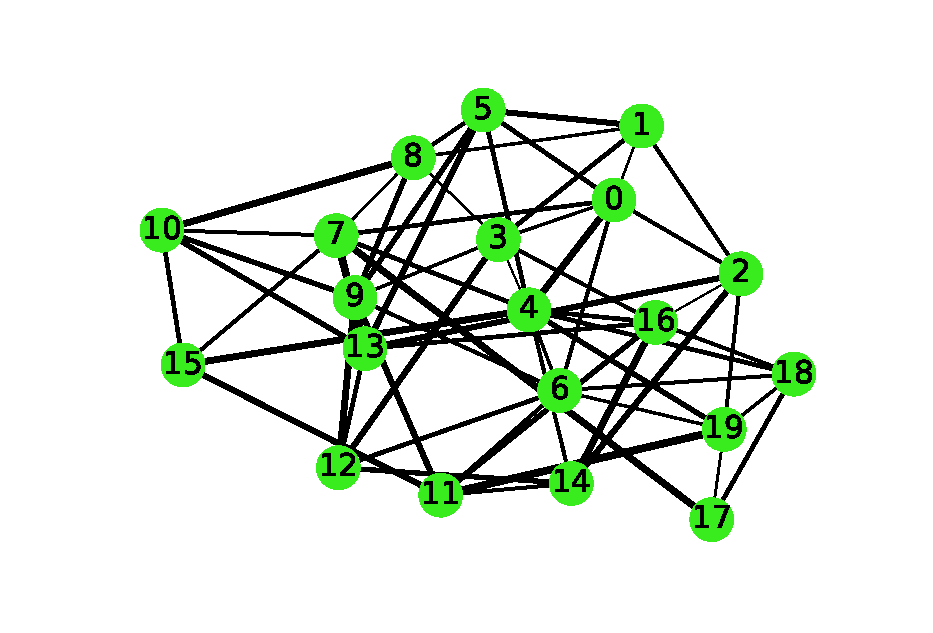
\includegraphics[scale=0.50]{fig5a.eps}}
\subfigure[\textit{Flujo máximo 82u }]{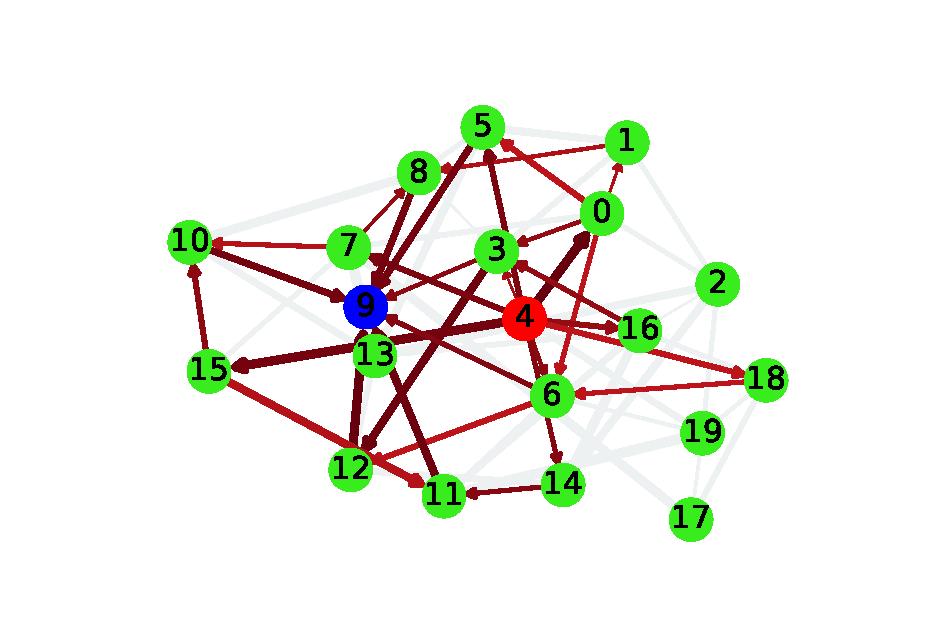
\includegraphics[scale=0.50]{fig5b1.eps}}
\subfigure[\textit{Flujo mínimo 33u }]{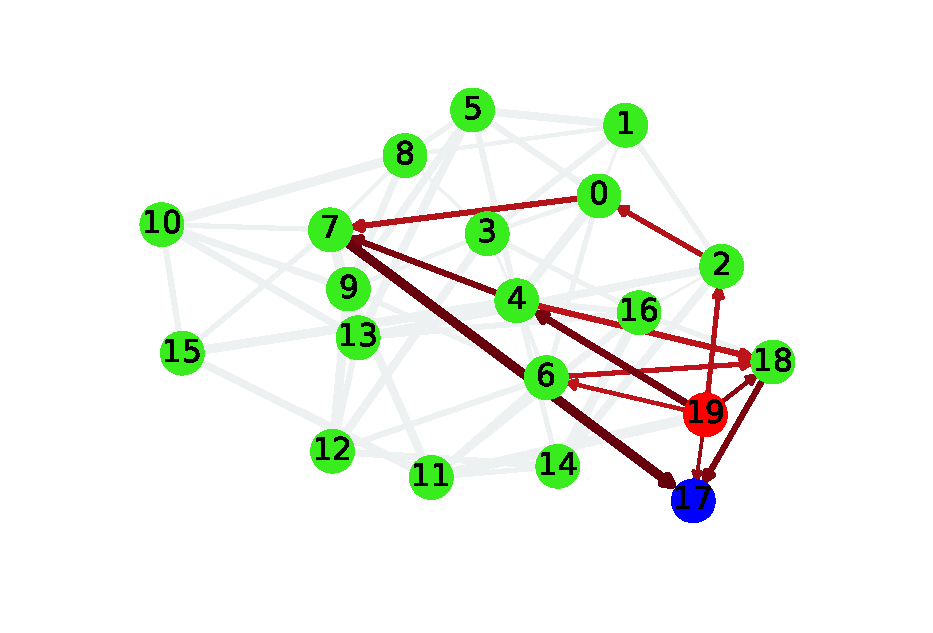
\includegraphics[scale=0.50]{fig5bpeor.eps}}
\caption{Variación de fuente y sumidero en grafo 5}
\label{Fig16} 
\end{figure}

Seguidamente se muestra el código empleado en esta sección
\newpage
\lstinputlisting[language=Python, firstline=76, lastline=159]{T5ProTimeFLujo.py}.

\newpage
\section{Análisis de varianza (ANOVA) y prueba de \textit{Tukey} para determinar la relación entre las propiedades de los nodos y las variable dependientes estudiadas} 


Para realizar el análisis del comportamiento de la variables dependientes \textit{tiempo de ejecución} y \textit{flujo máximo} con respecto a cada factor a analizar se realizó un análisis de varianza (ANOVA) para cada factor.

En el caso de las propieddes que se usan como factores en el ANOVA se realizó un histograma para cada una de ellas de modo que se puediera llevar a escalas los valores de las mismas.

Los histogramas se emplean para establecer los rangos de valores asignándoles una etiqueta de bajo, medio y alto para cada propiedad.

El resultado del análisis ANOVA con respecto al tiempo de ejecución para cada propiedad se muestra en los cuadros del uno al seis.Según los resultados en todas las propiedas se rechaza la hipótesis nula por lo que todas influyen en el tiempo excepto la centralidad de carga de rango alto, en la que según los resultados obtenidos se acepta la hipótesis nula. Esto se puede corroborar al analizar los diagramas de cajas de cada una de las propiedades. Ver figura \ref{Fig8} de la página \pageref{Fig8}. Del análisis de los resultados se aprecia que el que menos influye es la centralidad de carga, como se observa también en los diagramas de caja y prueba de \textit{Tukey} (ver figura \ref{Fig9} de la página \pageref{Fig9}) el resto de las propiedades sí influyen en el tiempo de ejecución del algoritmo al variar los nodos fuentes y sumideros.   

% Table generated by Excel2LaTeX from sheet 'Tabla_ANOVATimeCentCarga'
\begin{table}[htbp]
  \centering
  \caption{ANOVA Centralidad de Carga}
    \begin{tabular}{lrrrlll}
    \textbf{Source} & \multicolumn{1}{l}{\textbf{SS}} & \multicolumn{1}{l}{\textbf{DF}} & \multicolumn{1}{l}{\textbf{MS}} & \textbf{F} & \textbf{p-unc} & \textbf{np2} \\
    \midrule
    CentCarga & 0     & 2     & 0     & \multicolumn{1}{r}{0.058} & \multicolumn{1}{r}{0.94360248} & \multicolumn{1}{r}{0} \\
    Within & 0.126 & 1897  & 0     & -     & -     & - \\
    \bottomrule
    \end{tabular}%
  \label{tab:addlabel}%
\end{table}%

% Table generated by Excel2LaTeX from sheet 'Tabla_ANOVATimeCentCercania'
\begin{table}[htbp]
  \centering
  \caption{ANOVA Centralidad de cercanía}
    \begin{tabular}{lrrrlll}
    \textbf{Source} & \multicolumn{1}{l}{\textbf{SS}} & \multicolumn{1}{l}{\textbf{DF}} & \multicolumn{1}{l}{\textbf{MS}} & \textbf{F} & \textbf{p-unc} & \textbf{np2} \\
    \midrule
    CentCercania & 0.024 & 2     & 0.012 & \multicolumn{1}{r}{221.416} & \multicolumn{1}{r}{3.76E-87} & \multicolumn{1}{r}{0.189} \\
    Within & 0.102 & 1897  & 0     & -     & -     & - \\
    \bottomrule
    \end{tabular}%
  \label{tab:addlabel}%
\end{table}%

% Table generated by Excel2LaTeX from sheet 'Tabla_ANOVATimeCoefAgrup'
\begin{table}[htbp]
  \centering
  \caption{ANOVA Coeficiente de agrupamiento}
    \begin{tabular}{lrrrlll}
    \textbf{Source} & \multicolumn{1}{l}{\textbf{SS}} & \multicolumn{1}{l}{\textbf{DF}} & \multicolumn{1}{l}{\textbf{MS}} & \textbf{F} & \textbf{p-unc} & \textbf{np2} \\
    \midrule
    CoefAgrup & 0.007 & 2     & 0.004 & \multicolumn{1}{r}{56.285} & \multicolumn{1}{r}{1.79E-24} & \multicolumn{1}{r}{0.056} \\
    Within & 0.119 & 1897  & 0     & -     & -     & - \\
    \bottomrule
    \end{tabular}%
  \label{tab:addlabel}%
\end{table}%

% Table generated by Excel2LaTeX from sheet 'Tabla_ANOVATimeDistGrado'
\begin{table}[htbp]
  \centering
  \caption{ANOVA Distribución de Grado}
    \begin{tabular}{lrrrlll}
    \textbf{Source} & \multicolumn{1}{l}{\textbf{SS}} & \multicolumn{1}{l}{\textbf{DF}} & \multicolumn{1}{l}{\textbf{MS}} & \textbf{F} & \textbf{p-unc} & \textbf{np2} \\
    \midrule
    DistGrado & 0.023 & 2     & 0.011 & \multicolumn{1}{r}{209.861} & \multicolumn{1}{r}{4.61E-83} & \multicolumn{1}{r}{0.181} \\
    Within & 0.103 & 1897  & 0     & -     & -     & - \\
    \bottomrule
    \end{tabular}%
  \label{tab:addlabel}%
\end{table}%

% Table generated by Excel2LaTeX from sheet 'Tabla_ANOVATimeExcentCarga'
\begin{table}[htbp]
  \centering
  \caption{ANOVA Excentricidad}
    \begin{tabular}{lrrrlll}
    \textbf{Source} & \multicolumn{1}{l}{\textbf{SS}} & \multicolumn{1}{l}{\textbf{DF}} & \multicolumn{1}{l}{\textbf{MS}} & \textbf{F} & \textbf{p-unc} & \textbf{np2} \\
    \midrule
    ExcentCarga & 0.013 & 2     & 0.006 & \multicolumn{1}{r}{104.776} & \multicolumn{1}{r}{6.90E-44} & \multicolumn{1}{r}{0.099} \\
    Within & 0.113 & 1897  & 0     & -     & -     & - \\
    \bottomrule
    \end{tabular}%
  \label{tab:addlabel}%
\end{table}%

% Table generated by Excel2LaTeX from sheet 'Tabla_ANOVATimePageR'
\begin{table}[htbp]
  \centering
  \caption{ANOVA \textit{PageRange}}
    \begin{tabular}{lrrrlll}
    \textbf{Source} & \multicolumn{1}{l}{\textbf{SS}} & \multicolumn{1}{l}{\textbf{DF}} & \multicolumn{1}{l}{\textbf{MS}} & \textbf{F} & \textbf{p-unc} & \textbf{np2} \\
    \midrule
    PageR & 0.01  & 2     & 0.005 & \multicolumn{1}{r}{82.216} & \multicolumn{1}{r}{5.72E-35} & \multicolumn{1}{r}{0.08} \\
    Within & 0.116 & 1897  & 0     & -     & -     & - \\
    \bottomrule
    \end{tabular}%
  \label{tab:addlabel}%
\end{table}%

\newpage
\begin{figure}[htbp]
\subfigure[\textit{CentCarga}]{\includegraphics[scale=0.30]{Imagenes/aboxplotCentCarga.eps}}
\subfigure[\textit{CentCercania}]{\includegraphics[scale=0.30]{Imagenes/aboxplotCentCercania.eps}}
\subfigure[\textit{CoefAgrup}]{\includegraphics[scale=0.30]{Imagenes/aboxplotCoefAgrup.eps}}
\subfigure[\textit{aboxplotDistGrado}]{\includegraphics[scale=0.30]{Imagenes/aboxplotDistGrado.eps}}
\subfigure[\textit{Excent}]{\includegraphics[scale=0.30]{Imagenes/aboxplotExcentCarga.eps}}
\subfigure[\textit{PageR}]{\includegraphics[scale=0.30]{Imagenes/aboxplotPageR.eps}}
\caption{Diagrama de caja del ANOVA con Tiempo}
\label{Fig8} 
\end{figure}

Los resultados \textit{Tukey} de este análisis se muestran en la figura \ref{Fig9} de la página \pageref{Fig9} 

\begin{figure}[htbp]
\subfigure[\textit{CentCarga}]{\includegraphics[scale=0.3, trim=0 0 0 20, clip=true]{Imagenes/tablatukeyTimeCentCarga.eps}}
\subfigure[\textit{CentCercania}]{\includegraphics[scale=0.3, trim=0 0 0 20, clip=true]{Imagenes/tablatukeyTimeCentCercania.eps}}
\subfigure[\textit{CoefAgrup}]{\includegraphics[scale=0.3, trim=0 0 0 20, clip=true]{Imagenes/tablatukeyTimeCoefAgrup.eps}}
\subfigure[\textit{aboxplotDistGrado}]{\includegraphics[scale=0.3, trim=0 0 0 20, clip=true]{Imagenes/tablatukeyTimeDistGrado.eps}}
\subfigure[\textit{Excent}]{\includegraphics[scale=0.3, trim=0 0 0 20, clip=true]{Imagenes/tablatukeyTimeExcentCarga.eps}}
\subfigure[\textit{PageR}]{\includegraphics[scale=0.3, trim=0 0 0 20, clip=true]{Imagenes/tablatukeyTimePageR.eps}}
\caption{Diagrama de TUKEY para ANOVA con Tiempo}
\label{Fig9} 
\end{figure}
\newpage
Al realizar el análisis ANOVA para verificar la influencia de las propiedades en el flujo máximo se obtuvieron los resultados que se muestran en los cuadros del 7 al 12. En los mismos se aprecia que se rechaza la hipótesis nula en todos los casos excepto en la propiedad de centralidad de carga en la que se acepta la hipótesis nula. Se incluyen los diagramas de caja (ver figura \ref{Fig10} de la página \pageref{Fig10}) y las pruebas de \textit{Tukey} para profundizar en los resultados (ver figura \ref{Fig11} de la página \pageref{Fig11}). Se observa que la propiedad que menos influye es la centralidad de carga para valores altos, el resto de las propiedades sí influye al variar los nodos fuestes y sumideros en el valor de flujo máximo.



% Table generated by Excel2LaTeX from sheet 'Tabla_ANOVAflujomaxCentCarga'
\begin{table}[htbp]
  \centering
  \caption{ANOVA flujo max CentCarga}
    \begin{tabular}{lrrrlll}
    \textbf{Source} & \multicolumn{1}{l}{\textbf{SS}} & \multicolumn{1}{l}{\textbf{DF}} & \multicolumn{1}{l}{\textbf{MS}} & \textbf{F} & \textbf{p-unc} & \textbf{np2} \\
    \midrule
    CentCarga & 0.471 & 2     & 0.236 & \multicolumn{1}{r}{2.473} & \multicolumn{1}{r}{0.08461665} & \multicolumn{1}{r}{0.003} \\
    Within & 180.834 & 1897  & 0.095 & -     & -     & - \\
    \bottomrule
    \end{tabular}%
  \label{tab:addlabel}%
\end{table}%

% Table generated by Excel2LaTeX from sheet 'Tabla_ANOVAflujomaxCentCercania'
\begin{table}[htbp]
  \centering
  \caption{ANOVA flujo max CentCercanía}
    \begin{tabular}{lrrrlll}
    \textbf{Source} & \multicolumn{1}{l}{\textbf{SS}} & \multicolumn{1}{l}{\textbf{DF}} & \multicolumn{1}{l}{\textbf{MS}} & \textbf{F} & \textbf{p-unc} & \textbf{np2} \\
    \midrule
    CentCercania & 68.685 & 2     & 34.343 & \multicolumn{1}{r}{578.476} & \multicolumn{1}{r}{7.16E-197} & \multicolumn{1}{r}{0.379} \\
    Within & 112.62 & 1897  & 0.059 & -     & -     & - \\
    \bottomrule
    \end{tabular}%
  \label{tab:addlabel}%
\end{table}%
% Table generated by Excel2LaTeX from sheet 'Tabla_ANOVAflujomaxCoefAgrup'
\begin{table}[htbp]
  \centering
  \caption{ANOVA flujo max CoefAgrup}
    \begin{tabular}{lrrrlll}
    \textbf{Source} & \multicolumn{1}{l}{\textbf{SS}} & \multicolumn{1}{l}{\textbf{DF}} & \multicolumn{1}{l}{\textbf{MS}} & \textbf{F} & \textbf{p-unc} & \textbf{np2} \\
    \midrule
    CoefAgrup & 19.784 & 2     & 9.892 & \multicolumn{1}{r}{116.181} & \multicolumn{1}{r}{2.53E-48} & \multicolumn{1}{r}{0.109} \\
    Within & 161.521 & 1897  & 0.085 & -     & -     & - \\
    \bottomrule
    \end{tabular}%
  \label{tab:addlabel}%
\end{table}%

% Table generated by Excel2LaTeX from sheet 'Tabla_ANOVAflujomaxDistGrado'
\begin{table}[htbp]
  \centering
  \caption{ANOVA flujo max DistGrado}
    \begin{tabular}{lrrrlll}
    \textbf{Source} & \multicolumn{1}{l}{\textbf{SS}} & \multicolumn{1}{l}{\textbf{DF}} & \multicolumn{1}{l}{\textbf{MS}} & \textbf{F} & \textbf{p-unc} & \textbf{np2} \\
    \midrule
    DistGrado & 68.851 & 2     & 34.426 & \multicolumn{1}{r}{580.732} & \multicolumn{1}{r}{1.77E-197} & \multicolumn{1}{r}{0.38} \\
    Within & 112.454 & 1897  & 0.059 & -     & -     & - \\
    \bottomrule
    \end{tabular}%
  \label{tab:addlabel}%
\end{table}%

% Table generated by Excel2LaTeX from sheet 'Tabla_ANOVAflujomaxExcentCarga'
\begin{table}[htbp]
  \centering
  \caption{ANOVA flujo max Excent}
    \begin{tabular}{lrrrlll}
    \textbf{Source} & \multicolumn{1}{l}{\textbf{SS}} & \multicolumn{1}{l}{\textbf{DF}} & \multicolumn{1}{l}{\textbf{MS}} & \textbf{F} & \textbf{p-unc} & \textbf{np2} \\
    \midrule
    ExcentCarga & 54.856 & 2     & 27.428 & \multicolumn{1}{r}{411.472} & \multicolumn{1}{r}{3.69E-149} & \multicolumn{1}{r}{0.303} \\
    Within & 126.45 & 1897  & 0.067 & -     & -     & - \\
    \bottomrule
    \end{tabular}%
  \label{tab:addlabel}%
\end{table}%

% Table generated by Excel2LaTeX from sheet 'Tabla_ANOVAflujomaxPageR'
\begin{table}[htbp]
  \centering
  \caption{ANOVA flujo max \textit{PageR}}
    \begin{tabular}{lrrrlll}
    \textbf{Source} & \multicolumn{1}{l}{\textbf{SS}} & \multicolumn{1}{l}{\textbf{DF}} & \multicolumn{1}{l}{\textbf{MS}} & \textbf{F} & \textbf{p-unc} & \textbf{np2} \\
    \midrule
    PageR & 40.988 & 2     & 20.494 & \multicolumn{1}{r}{277.069} & \multicolumn{1}{r}{2.70E-106} & \multicolumn{1}{r}{0.226} \\
    Within & 140.317 & 1897  & 0.074 & -     & -     & - \\
    \bottomrule
    \end{tabular}%
  \label{tab:addlabel}%
\end{table}%

\begin{figure}[htbp]
\subfigure[\textit{CentCarga}]{\includegraphics[scale=0.30]{Imagenes/aboxplotflujomaxCentCarga.eps}}
\subfigure[\textit{CentCercania}]{\includegraphics[scale=0.30]{Imagenes/aboxplotflujomaxCentCercania.eps}}
\subfigure[\textit{CoefAgrup}]{\includegraphics[scale=0.30]{Imagenes/aboxplotflujomaxCoefAgrup.eps}}
\subfigure[\textit{aboxplotDistGrado}]{\includegraphics[scale=0.30]{Imagenes/aboxplotflujomaxDistGrado.eps}}
\subfigure[\textit{Excent}]{\includegraphics[scale=0.30]{Imagenes/aboxplotflujomaxExcentCarga.eps}}
\subfigure[\textit{PageR}]{\includegraphics[scale=0.30]{Imagenes/aboxplotflujomaxPageR.eps}}
\caption{Diagrama de caja del ANOVA con flujo máximo}
\label{Fig10} 
\end{figure}

\begin{figure}[htbp]
\subfigure[\textit{CentCarga}]{\includegraphics[scale=0.3, trim=0 0 0 20, clip=true]{Imagenes/tablatukeyflujomaxCentCarga.eps}}
\subfigure[\textit{CentCercania}]{\includegraphics[scale=0.3, trim=0 0 0 20, clip=true]{Imagenes/tablatukeyflujomaxCentCercania.eps}}
\subfigure[\textit{CoefAgrup}]{\includegraphics[scale=0.3, trim=0 0 0 20, clip=true]{Imagenes/tablatukeyflujomaxCoefAgrup.eps}}
\subfigure[\textit{aboxplotDistGrado}]{\includegraphics[scale=0.3, trim=0 0 0 20, clip=true]{Imagenes/tablatukeyflujomaxDistGrado.eps}}
\subfigure[\textit{Excent}]{\includegraphics[scale=0.3, trim=0 0 0 20, clip=true]{Imagenes/tablatukeyflujomaxExcentCarga.eps}}
\subfigure[\textit{PageR}]{\includegraphics[scale=0.3, trim=0 0 0 20, clip=true]{Imagenes/tablatukeyflujomaxPageR.eps}}
\caption{Diagrama de TUKEY para ANOVA con flujo máximo}
\label{Fig11} 
\end{figure}
\newpage
\bibliography{Referencias5}
\bibliographystyle{plainnat}
\end{document}

